\chapter{Quantifying the security benefits of debloating web applications}
\label{chap:lim}

\section*{Preamble}
Web application exploitation is unique in many ways compared to the binary exploitation. 
Common web application vulnerabilities (XSS, SQL injection, etc.) are orthogonal to data-only attacks on the binaries~\cite{ispoglou2018block}. 
As a result, removing dead-code which consists of code pieces that are unreachable from all entry points, provides marginal security benefits, since attackers cannot control the flow of execution in web applications through common exploits. 

Identifying this detail, we focused on modelling of code bloat as parts of the application (i.e., files, or functions) that are unused from the perspective of their users. 
To that end, we built synthetic models of usage behavior through encoding online tutorials of popular web applications as a means to model common tasks that the users perform. 
We then augmented this model by incorporating automated crawlers and testing mechanisms to further expand the code coverage of the web applications. 

Based on this modelling of the usage behavior, we characterized the main sources of bloat to be the third-party dependencies and unused modules and obscure features in web applications. 
We then proposed source-code based (i.e., reduction in logical lines of code, and code complexity~\cite{gill1991cyclomatic}) and security based (i.e., removal of CVEs, and object injection gadget) as metrics to quantify the security benefits of debloating. 

The remainder of this chapter is replicated from the paper titled ``Less is More: Quantifying the Security Benefits of Debloating Web Applications'' which was published in the proceedings of the 28th Usenix Security Symposium in 2019. 

\section*{Less is More: Quantifying the Security Benefits of Debloating Web Applications}

\subsection*{Abstract}

As software becomes increasingly complex, its attack surface expands enabling
the exploitation of a wide range of vulnerabilities. Web applications are no
exception since modern HTML5 standards and the ever-increasing capabilities
of JavaScript are utilized to build rich web applications, often subsuming
the need for traditional desktop applications. One possible way of handling
this increased complexity is through the process of software debloating, i.e.,
the removal not only of dead code but also of code corresponding to features
that a specific set of users do not require. Even though debloating has been
successfully applied on operating systems, libraries, and compiled programs,
its applicability on web applications has not yet been investigated.

In this paper, we present the first analysis of the security benefits of
debloating web applications. We focus on four popular PHP applications and
we dynamically exercise them to obtain information about the server-side code
that executes as a result of client-side requests. We evaluate two different
debloating strategies (file-level debloating and function-level debloating)
and we show that we can produce functional web applications that are 46\%
smaller than their original versions and exhibit half their original cyclomatic
complexity. Moreover, our results show that the process of debloating removes
code associated with tens of historical vulnerabilities and further shrinks
a web application's attack surface by removing unnecessary external packages
and abusable PHP gadgets.

%Use of rich web applications is becoming more widespread these days, as we move our complex systems to the web, we face different types of attack vectors and complex systems are harder to test, debug and reason about. One solid line of defense against exploitation has always been attack surface reduction, by limiting access to unnecessary services we can potentially prevent attackers from exploiting vulnerabilities in them. In this paper, we talk about a concept well known in binary world but less studied in the context of web. Software debloating is the process of removing code that is not necessary, e.g., instrumented by specific subset of users.

%First, we analyze four popular PHP web applications* top map known vulnerabilities to parts of code that results them, the chosen web applications span over four main web application categories namely, Administration tools, Wikis, CMSs and Online Shops. Second step is to dynamically analyze the applications to see if vulnerable lines of code are fired during user interaction. To address that, we create automation script to perform the tasks mentioned in online tutorials of those applications. To come up with a representative profile of general users of each application we enhance the code coverage from tutorials with the coverage from spiders that crawl web applications and monkey tests that try to brute force every possible action within the application. Third, based on the coverage resulted from tests in step two, we measure the coverage of code paths that intersect with known vulnerable lines. Arguably, if most users of an application do not use a feature, that feature can be removed, hence, removing the vulnerabilities within it.

%\todo{(Finalize numbers)} Our results show that on average we can remove \%75 of vulnerabilities by removing functions that do not fire during general use of users.  Debloating strategies can vary by their level of aggression and how far we want to go in terms of removing code from our application. By removing functions from studied web applications that would not be used by users of an application, we can significantly reduce the attack surface. In addition to the results, we open source our framework to record the coverage of individual lines within a web application under different usage profiles and automatically debloat the application under file and function level debloating conditions.

\section{Introduction}

% Web is important, becomes more complicated as well as more capable over time

Despite its humble beginnings, the web has evolved into a full-fledged
software delivery platform where users increasingly rely on web applications
to replace software that traditionally used to be downloaded and installed on
their devices. Modern HTML5 standards and the constant evolution of JavaScript
enable the development and delivery of office suites, photo-editing software,
collaboration tools, and a wide range of other complex applications, all
using HTML, CSS, and JavaScript and all delivered and rendered through the
user's browser.


This increase in capabilities requires more and more complex server-side
and client-side code to be able to deliver the features that users have
come to expect. However, as the code and code complexity of an application
expands, so does its attack surface. Web applications are vulnerable to
a wide range of client-side and server-side attacks including Cross-Site
Scripting~\cite{xss,kirda2006noxes,vogt2007cross}, Cross-Site
Request Forgery~\cite{csrf,jovanovic2006preventing,barth2008csrf},
Remote Code Execution~\cite{rce}, SQL
injection~\cite{sqlInjection,halfond2006classification}, and timing
attacks~\cite{brumley2003timing,vangoethem2015timing}. All of these
attacks have
been abused numerous times to compromise web servers, steal user data,
move laterally behind a company's firewall, and infect users with malware
and cryptojacking scripts~\cite{minesweeper-ccs2018, wang2018seismic,
cryptojacking-ccs2018}.

One possible strategy of dealing with ever-increasing software complexity is to
customize software according to the environment where it is used. This idea,
known as \textit{attack-surface reduction} and \textit{software debloating},
is based on the assumption that not all users require the same features from
the same piece of software. By removing the features of different deployments
of the same software according to what the users of each deployment require,
one can reduce the attack surface of the program by maintaining only the
features that users utilize and deem necessary. The principle of software
debloating has been successfully tried on operating systems (both to build
unikernel OSs~\cite{madhavapeddy2013unikernels} and to remove
unnecessary code from the Linux kernel~\cite{kurmus2013attack,
Kurmus:2011:ASR:1972551.1972557}) and more recently on shared
libraries~\cite{mishra2018shredder,quach2018debloating} and compiled binary
applications~\cite{heo2018effective}.

In this paper, we present the first evaluation of the applicability of software
debloating for web applications. We focus on four popular open-source PHP
applications (phpMyAdmin, MediaWiki, Magento, and WordPress) and we map the CVEs of 69
reported vulnerabilities to the source code of each web application. We utilize
a combination of tutorials (encoded as Selenium scripts), monkey testing,
web crawling, and vulnerability scanning to get an \emph{objective} and \emph{
unbiased} usage profile for each application. By using
these methods to stimulate the evaluated web applications in combination with
dynamically profiling the execution of server-side code, we can precisely
identify the code that was executed during this stimulation and therefore
the code that should be retained during the process of debloating.

Equipped with these server-side execution traces, we evaluate two different
debloating strategies (file-level debloating and function-level debloating)
which we use to remove unnecessary code from the web applications and quantify
the security benefits of this procedure. Among others, we discover an average
reduction of the codebase of the evaluated web application of 33.1\% for
file-level debloating and 46.8\% for function-level debloating, with comparable
levels of reduction in the applications' cyclomatic complexity.
In terms of
known vulnerabilities, we remove up to 60\% of known CVEs and the vast majority
of PHP gadgets that could be used in Property Oriented Programming attacks
(the equivalent of Return-Oriented Programming attacks for PHP applications).

\noindent Overall, our contributions are the following:

\begin{itemize}
  \setlength\itemsep{0.5em}
\item We encode a large number of application tutorials as Selenium scripts which, in combination with monkey testing, crawling, and vulnerability scanning, can be used to objectively exercise a web application. Similarly, we map 69 CVEs to their precise location in the applications' source code to be able to quantify whether the vulnerable code could be removed during the process of debloating.

\item We design and develop an end-to-end analysis pipeline using Docker containers which can execute client-side, application stimulation, while dynamically profiling the executing server-side code.

\item We use this pipeline to precisely quantify the security benefits of debloating web applications, finding that debloating pays large dividends in terms of security, by reducing a web application's source code, cyclomatic complexity, and vulnerability to known attacks.

\end{itemize}

\noindent To motivate further research into debloating web applications and to ensure the reproducibility of our findings, we are releasing \emph{all} data and software artifacts.

\section{Background}
\label{sec:background}

\begin{figure*}[t]
  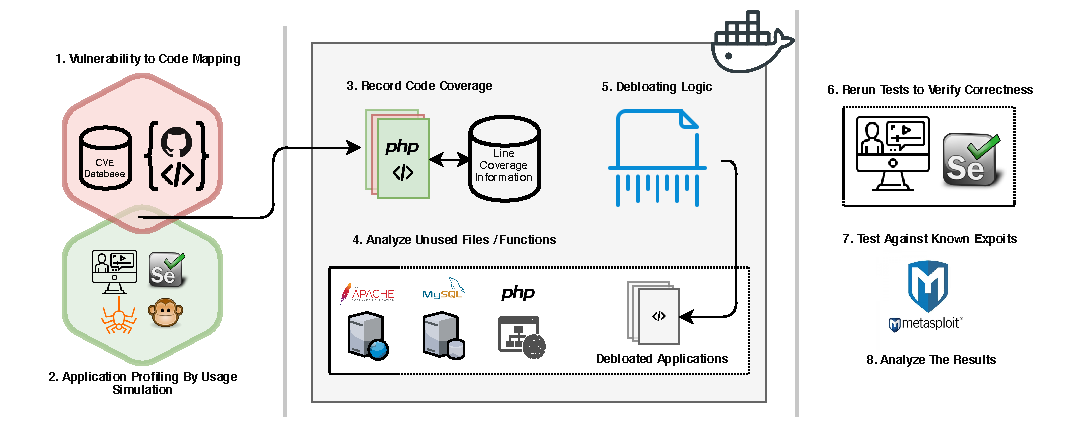
\includegraphics[width=\linewidth]{figures/lim/DebloatingPipeline.pdf}
  \vspace{-6ex}
  \caption{Overview of the architecture of our pipeline for debloating web applications and assessing the effects of different debloating strategies.}
  \vspace{-2ex}
  \label{fig:debloatingpipeline}
\end{figure*}

In this section, we briefly describe the effect of package managers on software
bloat and provide a motivating example for debloating web applications.


\subsection{Package managers and software bloat}
To ease the development of software, developers reuse third-party libraries,
external packages, and frameworks for their applications. This approach
enables developers to focus on their applications while relying on
proven and tested components. Statistics from popular package managers show
that reliance on external packages is a widely adopted practice across
many different languages. NPM, the registry hosting NodeJS packages,
reports more than 10 billion package downloads a
month~\cite{nodeDownloads}. Similarly, PyPI, the package manager for Python,
reports more than a billion a month~\cite{pypiDownloads}, while Packagist, the main repository for
Composer package manager for PHP, reports the download of 500 million
packages each month~\cite{packagistDownloads}.

At the same time, it is doubtful that \emph{all} the code and features
obtained through these packages and frameworks are actually used by
the applications that rely on them. For the most part, when developers rely on
external dependencies, they include entire packages with no effective way of
disabling and/or removing the parts of these packages and frameworks that
their applications do not require.

\subsection{Motivating web-application debloating}

In this study, we look at the bloat of web applications and quantify how
debloating can provide concrete security benefits. Even
though debloating has been successfully applied in other contexts, we argue
that the
idiosyncrasies of the web platform (e.g., the ambient authority of cookies and
the client/server model which is standard for the web but atypical
for operating systems and compiled software) require a dedicated analysis
of the applicability of debloating for web applications.

%As detailed in Section~\ref{sec:related}, several works have been
%published in the debloating domain but none of them looked specifically
%at web applications, nor did they tackle the subject from a security
%perspective. Indeed, web applications are vulnerable to different classes
%of attacks like code execution, denial of service or authentication bypass.
%Understanding the impact of debloating requires its own in-depth analysis
%that cannot be derived from other types of applications. Since we focus on
%the business logic of web applications, we decided upon PHP as the language
%used for this study. It is one of the most widely used server-side language
%in the world~\cite{phpAdoption} and very popular websites like Facebook,
%Yahoo or Wikipedia have a large part of their codebase written in this
%language. A package manager called Composer handles external dependencies
%in PHP~\cite{composer} and it relies on packages hosted on the Packagist
%website~\cite{packagist}.



To understand how the bloat of a web application can lead to a critical
vulnerability, we use a recent vulnerability of the Symfony web
framework (CVE-2018-14773~\cite{symfonyVulnerability}) as a motivating
example. Specifically, the Symfony web framework supported a legacy IIS
header that could be abused to have Symfony return a different URL than the
one in the request header, allowing the bypassing of web application firewalls
and server-side access-control mechanisms. If this type of header
was never used by the server, debloating the application would have removed
support for it, which ultimately would have prevented anyone from exploiting
the vulnerability. Drupal, a popular PHP Content Management System (CMS), was also affected by
the same vulnerability since it uses libraries from the Symfony framework
to handle parts of its internal logic~\cite{drupalVulenrability}. Even
if Drupal developers were not responsible for the code that leads to the
vulnerability, their application could still be exploited since Symfony
was an external dependency. Even more interestingly, an analysis of the
official Symfony patch on GitHub~\cite{symfonyPatch}
reveals that the vulnerable lines were derived from yet another framework
called Zend~\cite{zendVulnerability}. This shows that the structure of web
applications can be very complex with code reuse originating from many
different sources. Even if developers take all possible precautions to
minimize vulnerabilities in their own code, flaws from external dependencies
can cascade and lead to a critical entry point for an attacker.

Overall, there are clear benefits that debloating could have on web
applications. Assuming that we are able to pinpoint all the code that is required
by the users of a given software deployment, all other code (including the
code containing vulnerabilities) can be removed from that deployment.



\section{Setup}
In this section, we describe the process of gathering information regarding
known vulnerabilities (in the form of CVEs) for web applications, designing
and executing tests against web applications of interest, and identifying
the server-side code that was executed as a result of client-side actions.

\subsection{Overview}
The setup for our framework is depicted in
Figure~\ref{fig:debloatingpipeline}. To debloat target applications, we first
collect information about the vulnerabilities of the applications that we
analyze in our study. This information includes the files, functions, and
line numbers where each
vulnerability resides (Step 1, Section~\ref{sec:vulntosourcemapping}). Then,
we simulate usage of the application through a combination of different
techniques (Step 2, Section~\ref{subsec:profiling}). Using a PHP profiler
tool (\texttt{XDebug}), we record the lines, functions, and files, that are
triggered during the simulation (Step 3, Section~\ref{subsec:coverage}).

\begin{figure*}[t]
  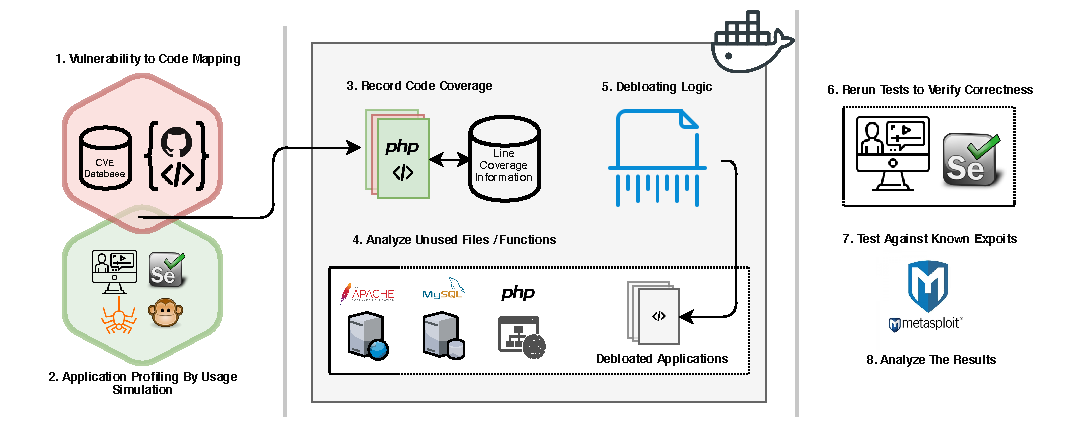
\includegraphics[width=\linewidth]{figures/lim/DebloatingPipeline.pdf}
  \caption{Overview of the architecture of our pipeline for debloating web applications and assessing the effects of different debloating strategies.}
  \label{fig:debloatingpipeline}
\end{figure*}

In the middle part of our pipeline, the debloating engine takes both the
target applications and coverage information to perform debloating at
different levels of granularity, and rewrite parts of the application to
remove unused pieces of code based on the debloating strategy being evaluated
(Steps 4 and 5, Section~\ref{sec:debloating}). Our framework also provides
a complete reporting panel to assist human analysts in understanding which
vulnerabilities can be removed by the present debloating strategies.

Last, we verify the correctness of our debloating process by running
a set of tests against the debloated web applications, and verifying that
no removed piece of code is triggered (Step 5). To this end, we
utilize assertions in place of the removed code blocks. An absence of error
messages from these assertions means that all tests were successfully
completed without triggering any missing server-side code. As a final step of
verification, we also test the debloated applications against a series of
exploits and verify that exploits which
abuse any of the vulnerabilities that were removed as part of the debloating
process, do not succeed (Step 6, Section~\ref{section:metasploit}).

To ease the integration and facilitate the analysis of new web applications, we
adopted a modular architecture that relies on three Docker containers. The
\textit{Application} container hosts our web applications.  The profiler
enabled on its web server is responsible for collecting code-coverage
information. The \textit{Database} container runs a MySQL server that
stores the code-coverage information along with the databases of the tested
applications. Lastly, the \textit{Debloating} container which includes our
debloating logic, analyzes the coverage information and generates debloated
versions of applications. It also provides a reporting panel that indicates
which vulnerabilities are removed in each application after debloating. To add
a new vulnerability, a user simply has to provide the details of the vulnerable
file(s) and line(s).

%In the end, this modular architecture makes the integration of our framework with new web applications and addition of new vulnerabilities seamless.


\subsection{Analyzed web applications}
\label{subsec:webapps}

%\begin{table*}[]
%\centering
%\caption{Analyzed open-source web applications and their corresponding versions.}
%\begin{tabular}{@{}lll@{}}
%%\toprule
%\textbf{Web Application}  & \textbf{Versions} \textit{(Release Date)}                                                                                  & \textbf{Known CVEs} \textit{($\geq$2013)}              \\ \midrule
%\multicolumn{1}{l}{Magento}                          & 1.9.0 \textsubscript{2014-5}, 2.0.5 \textsubscript{2016-4}                                                                             & 10                       \\ \midrule
%\multicolumn{1}{l}{MediaWiki}  & \multicolumn{1}{l}{1.19.1 \textsubscript{2012-06}, 1.21.1 \textsubscript{2013-05}, 1.23.0 \textsubscript{2014-06}, 1.24.0 \textsubscript{2014-11}, 1.28.0 \textsubscript{2016-11}} & \multicolumn{1}{l}{111} \\ \midrule
%\multicolumn{1}{l}{phpMyAdmin} & \multicolumn{1}{l}{4.0.0 \textsubscript{2013-05}, 4.4.0 \textsubscript{2015-04}, 4.6.0 \textsubscript{2016-03}, 4.7.0 \textsubscript{2017-03}}                      & \multicolumn{1}{l}{130} \\ \midrule
%\multicolumn{1}{l}{{Wordpress}}                          & {3.9.0 \textsubscript{2014-4}, 4.0 \textsubscript{2014-9}, 4.2.3 \textsubscript{2015-7}, 4.6 \textsubscript{2016-8}, 4.7 \textsubscript{2016-12}, 4.7.1 \textsubscript{2017-1}}                                                                             & {131}                       \\
%\bottomrule
%\end{tabular}
%\label{table:analyzed_webapps}
%\end{table*}

To understand how the process of debloating increases the security of web
applications, we decided against using toy-like web applications. Instead,
we focused on established open-source applications with millions of users,
and the presence of a sufficient number of known historical vulnerabilities
(in the form of CVEs) to allow us to generalize from them. To this end, we
selected {phpMyAdmin}~\cite{phpmyadmin},
{MediaWiki}~\cite{mediawiki}, {Magento}~\cite{magento}, and WordPress~\cite{wordpress},
which are representative samples of four different types of
web applications namely web-administration tools, wikis, online
shops, and blogging software. Table~\ref{table:analyzed_webapps} shows the versions of these web
applications that we utilized, in order to map CVEs to the location of the
vulnerability in the source code of each application.


%Initially, we study the registered CVEs for a subset of famous open source
%PHP applications. To capture different types of application architectures, we
%cover the following range of categories: \textit{``Web Administration Tools''}
%with phpMyAdmin, \textit{``Wiki''} with MediaWiki and \textit{``Online
%Shops''} with Magento. To map registered CVEs to the vulnerable piece
%of source code for each application, we used a set of versions for each
%application that contain the studied CVEs. These applications are listed
%in Table~\ref{table:analyzed_webapps}.
% We can refer to buildwith stats if we need to reason about why we chose these applications, both usage statistics and registered covers
% Why PHP: https://trends.builtwith.com/framework/programming-language
% Ecommerce: https://trends.builtwith.com/shop

\begin{table}[]
\centering
\caption{Analyzed open-source web applications.}
\scalebox{0.87}{
\begin{tabular}{|l|l|c|}
\hline
\textbf{Web Application} & \textbf{Version}                            & \begin{tabular}[c]{@{}l@{}}\textbf{Known CVEs}\\\hspace{1em}(2013-2019)\end{tabular} \\ \hline
Magento                  & 1.9.0, 2.0.5                                 & 10                                                                     \\ \hline
MediaWiki                & 1.19.1, 1.21.1, 1.24.0, 1.28.0 & 111                                                                    \\ \hline
phpMyAdmin               & 4.0.0, 4.4.0, 4.6.0, 4.7.0     & 130                                                                    \\ \hline
WordPress                & 3.9.0, 4.0, 4.2.3, 4.6, 4.7, 4.7.1  & 131                                                                    \\ \hline
\end{tabular}
}
\label{table:analyzed_webapps}
\end{table}

\subsection{Vulnerability to source-code mapping}
\label{sec:vulntosourcemapping}
To determine whether debloating web applications can actually remove
vulnerabilities, we performed a mapping of known CVEs to the vulnerable lines,
functions, and files, that they exploit in each application. This way, by
looking at an application after debloating, we can determine if the files,
functions, or lines responsible for the vulnerability, are still present or
were removed during the debloating process.


Even though there exist multiple databases listing the current and
historical CVEs of popular software (including the web applications in
question)~\cite{cvedetails,nistgov}, locating the actual source code
containing the vulnerability described in a CVE, is a non-trivial process
which requires careful investigation. In some cases, the right patch can be
discovered because of a direct reference to a CVE in a commit message, or in
a bug report on official public repositories of web applications. For others,
the fix is included within numerous commits that have to be carefully analyzed
to locate the appropriate lines of code. Since a vulnerability can span over
multiple lines, functions, and even multiple files, we record all affected
locations in a database so that this information can be later correlated
with each evaluated application.

%\todo{The following paragraph seems out of place... perhaps something for
%the background section}
%The premise behind debloating is that vulnerabilities exist in parts of a
%program that are never used in specific deployments of interest, and therefore
%can be safely removed (i.e., debloated). This makes the success of debloating
%highly dependent on the usage profile of an application and the location of
%any given vulnerability.
%%In the end, as debloating is based on specific usage profile, some
%%vulnerabilities may be more frequently mitigated than others depending on their
%%location in the source code. If a vulnerability belongs to a feature within
%%the application that is rarely triggered by normal users or that is hidden
%%behind privileged access, they may often be removed from the source code.
%To understand this better, we cam investigate a specific example of critical
%vulnerability. CVE-2016-6620 is a PHP object injection vulnerability that
%affects phpMyAdmin 4.6.0. It has a CVSS score of 9.8 which represents a highly
%severe and critical vulnerability inside phpMyAdmin. It consists of calling
%the PHP \textit{unserialize} function with unsanitized user-supplied data
%which then leads to code execution upon deserialization. This vulnerable
%feature has to be manually enabled by the user and is not part of the
%default configuration of phpMyAdmin. Hence, most usage profiles from real
%users will likely not contain any calls to this PHP \textit{unserialize}
%function, allowing the vulnerable code to be safely removed.


Given the time-consuming nature of mapping CVEs to existing code, for
this study, we limited ourselves to, at most, 20 CVEs per application
of interest.
The complete list of CVEs we mapped for this study can be found in
Table~\ref{table:listofallcves} in the Appendix.
To select these CVEs, we ordered existing vulnerabilities by
their CVSS score (thereby selecting the ones that are the most critical)
and we did not consider vulnerabilities that were reported before 2013. This
focus on fairly recent vulnerabilities (i.e., in the last five years) makes
our results more generalizable to the current state of web applications,
as opposed to quantifying vulnerabilities in source-code which has since
dramatically evolved. Note that, because not all versions of a web application
are vulnerable to all evaluated CVEs, we had to map vulnerabilities
across a number of different versions, as shown in
Table~\ref{table:analyzed_webapps}.



\subsection{Application usage profiling}
\label{subsec:profiling}

Modern web applications provide an incredibly wide range of features and
options to their users. Even though, from a functional perspective, more
features are desirable, from a security perspective, the code that implements
new features may contain new vulnerabilities thereby further expanding
a program's attack-surface. In order for a system to be
able to remove code related to unnecessary features, one must first identify
which features are necessary for a target set of users.

Given a usage profile, the goal of our framework is to produce debloated
versions of web applications which maintain the code and features that are
part of that profile but remove the rest. To be as objective as possible with
what features are considered ``necessary,'' we utilize four independent
sources of web application usage: i) online tutorials describing how to use
the applications of interest, ii) web crawlers that autonomously navigate
the application, iii) vulnerability scanners that feed malicious content to the
application, and iv) monkey testing tools that click on random parts of webpages
and type random keystrokes. The combination of all four gives our profiles
both breadth (through the crawler and monkey testing) as well as depth (through
the user following complicated paths while providing expected inputs and the
vulnerability scanner which provides large amounts of malicious inputs trying
to exploit the web application).

%In order to test our pipeline for this study, we created our own usage profile from scratch by using a combination of different automated techniques.
%First, to cover the core features of our tested web applications, we followed online tutorials and wrote Selenium tests based on them.
%This way, we obtain replayable tests that trigger the most essential lines in an application.
%Then, to augment coverage and add easy-to-reach options that are likely to be triggered, we used two additional techniques: spider software that can crawl the pages of the application interface and submit forms, and monkey testing scripts that click on random locations on the screen and type random keystrokes.
%While following the tutorials covers key functionalities within the application, monkey and spider tests add more breadth to our coverage.


%Different users use different parts of web applications, this can be a result of an access restriction model or be based on the need of different users. Specialized applications will have their unique usage profile as studied by [cite the paper that studies usage profile of industry application]. In our model, we simulate a general user that installs the application and uses available online tutorials to find his way through the applications. To that end, we automated the tutorials for our target web applications using selenium, to augment the coverage and add easy to reach options that the users are likely to trigger, we used spider software that would crawl the pages of the website and submit forms in addition to a monkey testing script that would click on random locations on the screen and type random keystrokes. While following the tutorials covers deep functionalities within the application, monkey and spider tests add more breadth to our coverage.

\subsubsection{Tutorials}
\label{sec:tutorials}
To simulate common interactions with an application, we use a popular search
engine to search for the application's name followed by the word ``tutorials''
(e.g., ``phpMyAdmin tutorials'') and follow the tutorials from the first two
pages of search results.

Specifically, we map each tutorial to a Selenium script that allows us to
both execute the same tutorial multiple times and also assess the correctness
of the results (e.g., encode that when we delete a database using phpMyAdmin,
the deleted database is no-longer shown in the list of databases). Note that
this mapping of tutorials to Selenium scripts is yet another time-consuming
process which, occasionally, has to be repeated for different versions of
the same web application. One change in a form field or in a selector can
break the complete flow of a test suite, and we observed a significant number
of cases with slight interface changes between two consecutive versions of
the same application.

Overall, after fine-tuning the scripts for all our tested versions, we obtained
46 tutorials which translated into 302 use cases scripted as Selenium tests
requiring 16,025 lines of code. Given our desire for complete reproducibility
of our results, we include the complete list of tutorials in the Appendix
(Table~\ref{table:listoftutorials}) along with WebArchive links that will
remain available despite potential future domain expirations and linkrot of
the original URLs~\cite{koehler2004longitudinal}.

%Tutorials model the behavior of the vast majority of users who try
%to setup the minimum necessary functionalities of applications and start
%working with them.
%While this approach triggers benign and valid use cases of the applications, it
%does not run code paths that lead to invalid inputs and does not cover the code
%for error handling.

Below, we provide a non-exhaustive list of actions that were part of the followed tutorials of each web application. 
% Full details are available in the actual tutorials and in the Selenium scripts which we will release together with this paper.
\vspace{0.5ex}

\noindent \textbf{Actions covered by phpMyAdmin tutorials:} As a web administration tool, all phpMyAdmin functionality is protected by an authentication mechanism.
We followed the actions described by tutorials when logged in as a root user account with full application access. The Selenium-encoded tutorials cover database operations including creating and dropping databases, filling tables with data, querying, table indexes, and importing/exporting data.
They also include administration tasks such as adding new user accounts, optimizing databases, checking database server status, obtaining performance metrics, and accessing server settings such as variables, charsets, and engines.

\vspace{0.5ex}

\noindent \textbf{Actions covered by MediaWiki tutorials:} MediaWiki provides different features depending on the privileges of the user.
Unauthenticated users can only visit and search pages.
Registered ones can post and edit content while administrators can perform moderation and management operations.
The tutorials that we followed cover all these different use cases.
More specifically, actions coded in our tutorials include authentication, creating and renaming pages, importing and exporting content from the wiki, as well as changing settings such as skins, styles, and formatting options.
%Modifying the navigation menu is a task that can only be performed by an administrator and is also covered by the tutorials. Finally, the tutorials also cover the importing and exporting content from the wiki.

\vspace{0.5ex}

\noindent \textbf{Actions covered by WordPress tutorials:} As a blogging software, WordPress has two distinct entry points, one for normal unauthenticated users to read blogs and post comments, and a separate administration panel accessible to privileged and authenticated users.
WordPress tutorials mostly focus on administrative tasks since normal users have limited abilities. The Selenium-encoded tutorials include actions such as creating a new post using HTML for the content, modifying most post options (ranging from visibility and tags to setting featured images), as well as downloading and changing WordPress themes.
%They cover different settings and include the managing of categories and tags.
For the administration panel, the tutorials include exporting content, setting up user accounts, and uploading media. Finally, the tutorials include the visiting of posts and the posting of comments as well as the management of comments, such as approving them, marking them as spam, and deleting them.
\vspace{0.5ex}

\noindent \textbf{Actions covered by Magento tutorials:} Magento is the largest evaluated web application in terms of source code and has the most features compared to the other applications. Similar to WordPress, the tutorials mostly target administration tasks which include store settings, advanced product search options, order notification via RSS, product pricing, currencies and tax rules, delivery and payment methods, emails and notifications, reviews and ratings and cache control. Some tutorials go in even more details by covering product and stock management, managing customers and groups configurations, modifying the UI, creating pages, and using widgets.
On the customer side, we followed tutorials that included registration of a new account, authentication actions, and purchasing products until checkout.






\subsubsection{Monkey testing}
\label{sec:monkey}
Monkey testing is a method for testing
software where the simulated user sends random clicks and keystrokes to the
target application. This unpredictable behavior can uncover bugs in an
application as it can trigger paths and actions that were not anticipated by
developers. In our case, we use such a technique to trigger additional code,
not covered by tutorials. We observe that this approach adds breadth to the
code-coverage by reaching easy to access features. In addition, by feeding
random keystrokes into forms, monkey testing can bring the application in an
error state thus exercising error-handling pieces of code.

We rely on the stress-testing library called
\texttt{gremlins.js}~\cite{gremlinsjs} in conjunction with the GreaseMonkey
browser extension~\cite{greasemonkey} to inject the library into web
application pages.
%During pilot stages of these experiments, we experimented
%with different configurations for \texttt{gremlins.js} (in terms of its
%combinations of Click, Scroll, Keystroke, and Delays actions) and arrived
%at a configuration that exercised as much as possible of each tested web
%application.
Since this kind of testing can occasionally trigger unwanted actions, we have
to take necessary steps to stop them, e.g., prevent the test from leaving
the web application and visiting external websites. We also want to prevent
\texttt{gremlins.js} from getting trapped on a single page as an unexpected
JavaScript
%\texttt{alert} or \texttt{prompt}
dialogue box or a dead end page can pause our test
execution.  %or the monkey can get stuck on a deadend page.
An additional issue is that of accidentally logging out a web application by
clicking on a logout link. Given that we run monkey-testing under three different
usage profiles (public user, logged-in user, and administrator) we took steps
to avoid accidental logouts. Overall, we perform the following
modifications: i) we remove all links that lead to external pages, ii) we
remove logout buttons for applications that require authentication, iii) we
override the aforementioned JavaScript functions and iv) we set a timeout to
detect when the monkey is stuck and reset it to a known good state. All these
actions are done using injected JavaScript on target pages prior to starting
the \texttt{gremlins.js} library.

To cover a large set of pages from a web application, we run
\texttt{gremlins.js} for 12 hours for each of the test profiles.
To guarantee the reproducibility of our experiment, we choose a fixed seed for
each run that will generate the same sequence of pseudo-random actions.


\subsubsection{Crawling}
Web spiders (also known as crawlers) are a type of bot that follows the
links of a web application and optionally submits forms with predefined
content. Each newly crawled page is added to a database of the application that
the crawler uses to prevent repeated visits to the same pages. For our study,
we use BurpSuite Spider v2.0.14~\cite{burpsuite} to crawl our web
applications. As a result, we augment the application coverage with code paths that were
not triggered, either through the followed tutorials or through monkey testing.

%Our results show that monkey testing and spiders produce different code-coverage and trigger different functionalities within tested applications. Hence, these two methods help us increase the diversity of our usage profiles.
%Hence, this is necessary to include both of these tests.

\subsubsection{Running vulnerability scanners}
Vulnerability scanners are tools that try to detect security flaws in web applications.
%In our case, the scanner increases our code-coverage by reaching unwanted states in the application.
We use BurpSuite Scanner v2.0.14~\cite{burpsuite} based on the URLs extracted by the spider to look for vulnerabilities in headers, URLs and forms.
Notably, the scanner tries different injection mechanisms like SQL injection, XSS, PHP file injection, and path traversal, to trigger errors and reach unwanted states in the application.
The vulnerability scanner goes beyond what the crawler and the monkey cover by modifying headers and URL parameters.
By inspecting the resulting coverage, we observe that each of these four methods result in exercising server-side code that would not have been exercised through the other methods. We quantify this relationship in Section~\ref{section:results}.


\subsection{Recording server-side code-coverage}
\label{subsec:coverage}

Regardless of the method that is used to interact with a web application,
in order to be able to successfully remove unused code (i.e., debloat the web
application), we must be able to
associate client-side requests with server-side code. To record the files
and lines of code that are triggered by user requests, we make use of PHP
profilers.

PHP profilers are available as PHP extensions that modify the PHP engine to
collect code-coverage information. There exist a number of different profilers,
such as, \texttt{XDebug}~\cite{XDebug}, \texttt{phpdbg}~\cite{phpdbg}, and
\texttt{xhprof}~\cite{xhprof} all of which require a similar setup to record
code-coverage. For our framework, we decided to use \texttt{XDebug} as it
is the most mature profiler and is actively maintained.

\subsubsection{Adding coverage support in a web application}

\vspace{1ex}
\noindent\textbf{Connecting a web application to XDebug.}
To be able to perform dynamic analysis and record lines of code
that are triggered by user requests, our framework must add calls
to specific \texttt{XDebug} functions in every PHP file of a web
application. Specifically, both \texttt{xdebug\_start\_code\_coverage()} and
\texttt{xdebug\_get\_code\_coverage()} functions are called to, respectively,
start and receive coverage information. If the ``get'' function is never
called, the coverage information is lost. In the following paragraphs, we
describe challenges related to obtaining the code-coverage from \texttt{XDebug}
and how we overcame them.

\vspace{1ex}
\noindent\textbf{The case of unrecorded lines.}
Boomsma and Gross reported on the possibility of removing unused code in a
custom PHP application~\cite{boomsma2012Dead}. By performing dynamic
analysis, they observed which files were not used and removed
them from their application. The authors utilized their own profiler and took
advantage of the \texttt{auto\_append} built-in function of PHP to add
the necessary log functions at the very end of all PHP files~\cite{autoappend}.

For our study, we initially attempted to use the same approach and ran
preliminary tests by appending \texttt{XDebug} function calls at the end
of our tested files. However, we discovered that the coverage was
incomplete and that some lines were not properly recorded. Given that any
PHP file can call the \textit{exit()} or \textit{die()} function at any
time to terminate the current script, our \texttt{XDebug} calls which were
located at the end of each file, were not always executed thus leading to
under-reported code-coverage.


%Since our ``xdebug\_get\_code\_coverage()'' calls were located at the very
%end of each PHP file, we were not able in some cases to collect the full
%coverage information because of these exit calls. For us to properly debloat
%our target web applications, we needed to go further.


\subsubsection{Main challenges for getting full coverage}
\label{subsubsec:challenges}

\vspace{1ex}
\noindent\textbf{Avoiding early exits.}
To overcome the coverage problems due to calls to exit functions, we
utilized a specific type of PHP callback functions, called \textit{shutdown}
functions. When registered, these functions are triggered after all the
code on the page has finished running or after either \textit{exit()} or
\textit{die()} functions are called. This way, we are able to obtain the
desired coverage information even if a PHP script used one of the aforementioned functions.
Interestingly, we also discovered that calls to \textit{exit()} inside a
shutdown function prevent the execution of other shutdown functions
including the call to collect our own code-coverage information. To correct
this issue, we statically analyzed the evaluated applications and automatically
added calls to collect code-coverage before these exit calls (e.g., Line 7
in Listing~\ref{listing:rewriting_webapps}).

\vspace{1ex}
\noindent\textbf{Getting correct coverage information of shutdown functions.}
Another challenge, in terms of recording correct code-coverage information,
is to properly record the executed lines of code inside shutdown functions. As
mentioned by the PHP manual~\cite{phpshutdown}, shutdown functions are called
in the order they were registered. This means that if our own shutdown function
is registered first, it will also be triggered first, thereby missing any
calls to subsequent shutdown functions present in the same PHP file. To get
full coverage, we use the following approach: our own shutdown function will
perform a late registration of a final shutdown function that will be added
at the very end of the execution queue. This way, we can be certain that
the very last shutdown function that will be executed in a script will be
our own, providing us with the desired coverage information.


\vspace{1ex}
\noindent\textbf{Getting correct coverage information of destructors.}
The final challenge that we faced was to properly record covered lines for
all class destructors. PHP uses garbage collection and reference counting to
remove objects from memory, whenever they are no longer necessary. However,
there is no real way to anticipate when the garbage collector will effectively
remove objects during program execution. If objects are destroyed \emph{before}
the shutdown functions are executed, our framework has no issue recording
them. However, if they are destroyed after, our shutdown functions are
incapable of registering the execution of these destructors.

To handle this special case, we rewrote class destructors so that they
register themselves while they are executing. Every time a destructor
is called, we query the \texttt{XDebug} engine to check whether code-coverage
recording is currently in progress. This way, we can determine whether the
destructor is called before or after shutdown functions. If the destructor
is called after shutdown functions, we dynamically decide to start recording
all executed lines within the destructor and save the coverage information
when it finishes executing.

%Every time a destructor is called, we query the XDebug engine to know if it was registered before.
%If it was not, we start recording all executed lines and save the coverage information when it finishes executing.

\begin{figure}[t]
  \begin{lstlisting}[frame=single, caption={Code rewritten by the debloating framework to ensure correct code-coverage of corner cases.},captionpos=b, label={listing:rewriting_webapps}]
  <?php
  register_shutdown_function("PMA_Response::resp");
  class PMA_Response {
    public static function resp() {
      $buffer->flush();
      // Prepend original call to exit:
      collect_code_coverage();
      exit;
    }
  }
  
  class TCPDF {
    public function __destruct() {
      // If called after shutdown_functions
      // start recording code-coverage
      ...
      // If called after shutdown_functions
      // stop coverage
    }
  }
  ?>
  \end{lstlisting}
\end{figure}

\vspace{1ex}
\noindent\textbf{Summary.}
%We use prepend and register shutdown functions
%we prepend before exit lines call to get coverage
As witnessed through the above use cases, collecting the correct code-coverage information
for a web application is significantly more complicated than one would
initially expect. Through the preprocessing of code, and the use of destructors
and shutdown functions, we solve the issues that were not even mentioned
in prior work and get a precise view of the code that executes at the server
side, as a result of user requests. Listing~\ref{listing:rewriting_webapps}
provides an example of concrete modifications in a PHP file. On line 7, we
added a code-coverage call before an \texttt{exit} which happens inside a shutdown functions to prevent information
loss due to early exits. On lines 14 and 17, we wrapped the destructor with
code-coverage calls.


%*****************************OLD
%\paragraph{Gathering coverage information when all PHP code has finished executing}
%In PHP, developers can register functions as ``shutdown\_functions'' that would be triggered by PHP engine after all the code on the page has finished running or after either \textit{exit()} or \textit{die()} functions are called.
%Our framework uses the same method to make sure ``xdebug\_get\_code\_coverage()'' is executed last.
%As described in the PHP language manual, if multiple shutdown\_functions are present, they will be executed in the same order that they are registered.
%
%At the same time, PHP scripts can call \textit{exit()} at any time during the execution.
%Architectures that use auto\_append to collect coverage information will miss the coverage for scripts that call \textit{exit()}.
%More interestingly, if this call to \textit{exit()} happens inside a shutdown\_function(), it will prevent the execution of other shutdown\_functions including the call to collect code-coverage information.
%
%\paragraph{code-coverage for PHP destructors} is another challenge that we have to overcome, PHP uses garbage collection and reference counting to remove objects from the memory. We can not reason about the exact time when destructors get executed. PHP object destruction order will call zend\_call\_destructors which then calls destructor functions of the remaining objects after shutdown\_functions are called.
%
%
%
%\subsubsection{Preparing web applications}
%\label{label:prep_software}
%Our framework statically analyzes web applications and rewrites their code to conform to our testing requirements mentioned in section~\ref{subsec:coverage}. Our three step solution to address issues mentioned in Section~\ref{subsec:coverage} uses a combination of preprocessing and programming hacks as depicted in Listing~\ref{listing:rewriting_webapps}.
%
%To make sure our call to collect the code-coverage is always executed, we statically analyze the applications and automatically prepend calls to \textit{exit()} with a call to collect code-coverage (Line 7). This way we make sure we have full coverage information before exiting and also do not change the original execution flow of applications.
%
%The second step is necessary to guarantee that our shutdown\_function which collects code-coverage information runs last. To achieve this, we register a second shutdown\_function within the first shutdown\_function and this trick makes sure the second registered function runs after all previously registered shutdown\_functions.
%
%Third step is to record code-coverage for all class destructors. We distinguish between two cases, destructors may execute before we stop recording code-coverage (i.e, before shutdown\_functions are called). In this case we do not need to do anything extra. But when destructors execute after after shutdown\_functions, we modify them to start recording code-coverage information and save this data after they finish executing. We track this state by querying XDebug engine to see if coverage recording is currently in progress and distinguish between the two cases. To handle this situation, our framework rewrites class destructors to call XDebug functions to record their coverage (Line 15 and 18 in Listing~\ref{listing:rewriting_webapps}).
%
%%One requirement is to make sure our function that collects code-coverage runs last, to do that we use shutdown\_functions. To prevent calls to \textit{die} or \textit{exit} before our shutdown\_function preventing its execution, our %framework preprocesses target web applications and rewrites such calls to make sure our shutdown\_function executes. Second requirement is to record code-coverage for destructors that run after shutdown\_functions, to that end the %framework rewrites destructors with proper calls to XDebug code-coverage functions.
%

\section{Debloating web applications}
\label{sec:debloating}

In this section, we briefly describe the evaluated debloating strategies and
the steps we took to ensure that the debloated applications remain functional.


\subsection{Debloating strategies}

By combining the simulated usage of a web application (achieved through
tutorials encoded in Selenium scripts, web crawlers, monkey testing, and
vulnerability scanning) with
server-side code profiling, we can identify the code that was executed
as part of handling web requests. Consequently, code whose execution was
not triggered by any client-side request can presumably be removed since
it is not necessary for any of the functionality that is desired by users
(as quantified by the utilized usage profiles).
In this work, we evaluate the following debloating strategies:
\vspace{-2ex}
\paragraph{$\bullet$ File-level debloating:} Given that the source code of web
applications spans tens or hundreds of different files, we can completely
remove a file, when none of the lines of code in that file were executed
during the stimulation of the web application.
\vspace{-2ex}
\paragraph{$\bullet$ Function-level debloating:} In function-level debloating, not
only can we remove entire files, but we can also selectively remove some of
the functions contained in other files. This is a more fine-grained approach
which allows us to remove more code, than the more conservative, file-level
debloating strategy.

%\begin{itemize}
%  \setlength\itemsep{0.5em}
%\item \textbf{File-level debloating:} Given that the source code of web
%applications spans tens or hundreds of different files, we can completely
%remove a file, when none of the lines of code in that file were executed
%during the stimulation of the web application.
%
%\item \textbf{Function-level debloating:} In function-level debloating, not
%only can we remove entire files but we can also selectively remove some of
%the functions contained in other files. This is a more fine-grained approach
%which allows us to remove more code, than the more conservative, file-level
%debloating strategy.
%\end{itemize}

More fine-grained approaches are possible, such as, the removal of specific code statements from retained functions which were not exercised during stimulation.
However, such changes essentially modify the logic of a function (e.g., removing
conditional code blocks) thereby increasing the probability of breaking the
resulting program when a minute change of a client-side request would lead the
execution into these blocks of code.
%{\color{blue} Moreover, recording the coverage of error handlers is a challenge that sub-function debloating mechanisms have to address. Error states that are not triggered during profiling will lead to the removal of such conditions and the final application will lack proper error handling upon receiving previously unseen requests.
%During the development of web applications, usually a function (e.g., a controller action in MVC architecture or its equivalent) contains the complete logic to handle the request. This standard architecture adopted by most web development frameworks relies on central error handling classes.
%This includes the code to handle proper execution of the function in addition to the code to handle errors. Even though this logic can be separated into different functions and classes,
%the decision to keep or remove the function does not break this chain.
%As such, we consider this level of debloating as out of scope, and leave its evaluation for future work.}


\subsection{Detecting the execution of removed code}


We replace all removed functions and files with placeholders which, if executed,
have the following tasks:
\vspace{-2ex}
\paragraph{$\bullet$ Exit the application:} If a placeholder happens to be triggered,
the PHP application will start its shutdown procedures. This way, the
application does not enter an unexpected state that was not planned by the
debloating process.
\vspace{-2ex}
\paragraph{$\bullet$ Record information about the missing function:} In order
to better understand which missing placeholders were triggered and how,
our framework logs several pieces of information, such as, the URL that
triggered the execution of the removed code, the name of the class and
function of the removed code, and the
corresponding line numbers.

%\begin{itemize}
%  \setlength\itemsep{0.5em}
%\item \textbf{Exit the application:} If a placeholder happens to be triggered,
%the PHP application will start its shutdown procedures. This way, the
%application does not enter an unexpected state that was not planned by the
%debloating process.
%
%\item \textbf{Record information about the missing function:} In order
%to better understand which missing placeholders were triggered and how,
%our framework logs several pieces of information, such as, the URL that
%triggered the execution of the removed code, the name of the class and
%function of the removed code, and the
%corresponding line numbers.

%{\color{red}TODO:\item \textbf{Proactively preventing required code from being removed:} Certain actions within web applications are not triggered by users and %sometimes specific actions need to run at certain intervals. Regardless of
%the entity triggering the action, our system is able to record its coverage. But if the interval to run the action is longer than the interval that record the code %coverage is recorded, the underlying code for that feature will be removed.

%**I'm not sure into how much detail I want to go here, shall I open the can of worms and talk about update scripts? We haven't spend that much time discovering and %whitelisting these stuff.
%The main goal here is to introduce whitelisting for error handlers, config files and the files that we know we do not use often but they are still required.**
%}
%\end{itemize}

To ensure that the debloating process has preserved the functionality of
the debloated web application, we rerun all the Selenium-mapped tutorials and monkey scripts
after the debloating stage. If our placeholder code for removed files and
functions executes during this stage, this means that this code should not
have been removed.

This feedback mechanism proved invaluable during the development of
our framework since it helped us identify problems with our coverage
logic which in turn revealed the challenges that we described in
Section~\ref{subsubsec:challenges}.

%%%%%%%%%%%%%%%%%%%%%%%%%%%%%%%%%%%%%%%%%%%%%%%%%%%%%%

%\paragraph{Assertions} are used throughout our debloating logic, when we debloat a unit of code, we replace it with a placeholder that contains an assertion code. If debloated files or functions are triggered, this code will notify us via web server logs that one of the tests triggered a removed unit of code along with useful information such as referer header, the page which triggered the execution of removed code and class name, function name and line number of the removed piece of code. This information is then used to verify the correctness of our debloating when rerunning tests in verification step.
%
%To prevent unwanted side effects when executing web applications after debloating, these assertions and placeholders stop the code execution to prevent execution of code paths which include removed functions and files.


%%%%%%%%%%%% TO BE PUT IN THE RESULTS SECTION
%\subsection{Definition of vulnerability coverage}
%An exploitable vulnerability in a web application can be the result of multiple vulnerable lines, functions or files that together they create a chain that leads to an exploit. On one end an application developer might fail to apply sanitization function on untrusted input which affects only one line of code but the same bad practice can be spread over multiple files, on the other end a chain of vulnerabilities has to be present and be chained together to form an exploit for a registered CVE.
%
%For each vulnerability, when our usage profiles line coverage data overlaps with vulnerable lines, we call the vulnerability to be triggered by our usage profiles regardless of full or partial overlap. In that sense we take the conservative approach.
%
%An executable line within a PHP application is considered triggered if usage profiles execute that line. Similarly a function is considered to be covered if usage profiles execute the first executable line within that function. This definition is based on the logic of PHP compiler and Zend engine where we do not have a notion of functions directly and have to define functions as the line number of first executable statement within them. One the same note, we define a PHP file to be covered by usage profiles if at least one executable line within that file is triggered. Based on these definitions we propose debloating methods that can remove units of code not triggered by usage profiles.


%\subsection{Debloating strategies}
%Based on usage profile information, we define a baseline debloating method which only removes PHP files if non of the executable lines within those files are triggered. We also analyze the potential benefits from debloating strategies which can remove specific vulnerable lines within the web applications if the usage profiles do not cover those lines. All other debloating methods should perform between these bounds in terms of mitigated CVEs. Second debloating strategy we introduce debloats functions. Our experiments show that this strategy works just as good as more fine grained debloating strategies in terms of removed CVEs. Note that while previous usage profiles might show that users do not trigger specific units of code through normal usage, attackers can still trigger the code. Hence, the debloated code should handle this situation properly, this challenge makes fine grained debloating that modified individual executable lines more challenging. Table~\ref{table:debloating_bounds} shows the performance of debloating strategies on the analyzed web applications in terms of removed CVEs.
%
%\begin{table}[]
%\begin{tabular}{|l|l|l|l|}
%\hline
%Web Application & \begin{tabular}[c]{@{}l@{}}Total\\ CVEs\end{tabular} & \begin{tabular}[c]{@{}l@{}}Lowerbound/\\ Upperbound\end{tabular} & \begin{tabular}[c]{@{}l@{}}Function\\ Debloating\end{tabular} \\ \hline
%phpMyAdmin      & 20                                                   & 7/15                                                             & 13                                                            \\ \hline
%MediaWiki       & 21                                                   & 6/13?                                                            & 15                                                            \\ \hline
%Magento         & 8                                                    & x/x                                                              & x                                                             \\ \hline
%\end{tabular}
%\caption{Debloating performance bounds}
%\label{table:debloating_bounds}
%\end{table}
%
%
%\subsection{File level debloating}
%The baseline debloating strategy we discuss debloats PHP files that are not covered by usage profiles. On average this approach yields removal of UPDATE**\%25** of known CVEs and reduces code size by **Y** amount. This approach is the least aggressive approach with limited effectiveness.
%\subsection{Function level debloating}
%In this approach, our framework removes functions that are not covered by our usage profiles and replaces them with assertions. Our analysis proves this approach to have a performance close to the upper bound of debloating strategies (i.e, a debloating strategy that debloats individual lines) in terms of number of removed CVEs. While the side effects of removing functions are minimal compared to individual lines, the result turns out to be promising. As shown in Table~\ref{table:debloating_bounds}, function level debloating on average mitigates **UPDATE NUMBER** \%75 of known CVEs on target web applications.

\section{Results}
\label{section:results}

To assess the impact of debloating web applications, we analyze our results
from a number of different perspectives. First, we show the contributions of different application-profiling methods and then compute different metrics
to understand the effectiveness of debloating in terms of reducing the attack surface of our tested applications. Next, we focus on CVEs to determine whether
debloating can actually remove critical vulnerabilities. Then, we take
a closer look at the bloat introduced by external packages along with the
security implications that come with using this specific development practice.
Finally, we look at what has effectively been removed in debloated applications and test a number of exploits against the original and debloated versions of the evaluated web applications.
% we use clustering to find which parts of the application are more affected by debloating.


%Property Oriented Programing (POP) is an exploitation technique in PHP which works similar to ROP (Return Oriented %Programming) and is used to exploit POI vulnerabilities. In this technique, the attacker creates exploit gadgets from %available code in the applications. Each object within the chain performs malicious actions or prepares the environment for %execution of next object in the chain upon deserialization. Dahse et al. have studied automatic generation of such gadget %chains in \cite{Dahse:2014:CRA:2660267.2660363}.

\subsection{Tutorials vs. Monkey Testing vs. \\Crawling vs. Vulnerability Scanning}
As described in Section~\ref{subsec:profiling}, to ensure that we exercise web applications in an objective and repeatable way, we utilized tutorials, monkey testing, crawlers, and vulnerability scanners. Figure~\ref{fig:venncoverage} shows the coverage, in terms of server-side files, that each method obtained on the latest version of each web application in our testbed. We can clearly see that all four methods are required, with each method contributing differently for different web applications.
For example, tutorials trigger more files in Magento compared to other applications, while Spider covers most unique files in WordPress.

%For example, while monkey testing appears to be responsible for triggering the vast majority of source code in MediaWiki, it does not perform nearly as well for the %remaining two applications.

\subsection{Debloating by the numbers}
To evaluate the effectiveness of our two debloating strategies, we computed different metrics that provide
insights into what has actually been removed during the debloating process.


\subsubsection{Logical lines of code}
\label{subsubsec:lloc}
The size of a program positively correlates with the number of programming errors (i.e., bugs). According to McConnel~\cite{mcconnell2004code}, the industry average, at least in 2004, was to have between 1 and 25 bugs for every one thousands lines of code. Given the importance of the size of an application to its overall security, we start by estimating the reduction of the attack surface by looking at the
Logical Lines Of Code (LLOC, sometimes also called Effective Lines Of
Code). LLOC is intended to measure lines of code without comments, empty
lines and syntactic structure required by the programming language. LLOC
reduction is a robust and precise indicator of how much the volume of
the code was reduced.
Figure~\ref{fig:lloc} reports on the LLOC for all versions of the applications
we debloated.

\paragraph{Number of logical lines over time.}
Looking at the number of LLOC of the original applications, we can observe two different evolution behaviors.
For WordPress, the amount of code is stable and there is even a small decrease of 2\% of LLOC between versions 4.7 and 4.7.1.
For the other applications, we observe the opposite where the source code in the latest versions spikes, compared to the ones released just before them: 82\% LLOC increase for phpMyAdmin, 99\% for MediaWiki, and 171\% for Magento. By
analyzing the code of these newer versions in an attempt to understand their
sudden expansion in size, we discovered that these spikes can be attributed to
a change in development practices, namely the reliance on external packages.
As WordPress does not rely on external packages, it does not exhibit this kind of behavior. We
discuss the issue of relying on external packages in more detail in Section~\ref{subsec:external}.


\begin{figure}[t]
  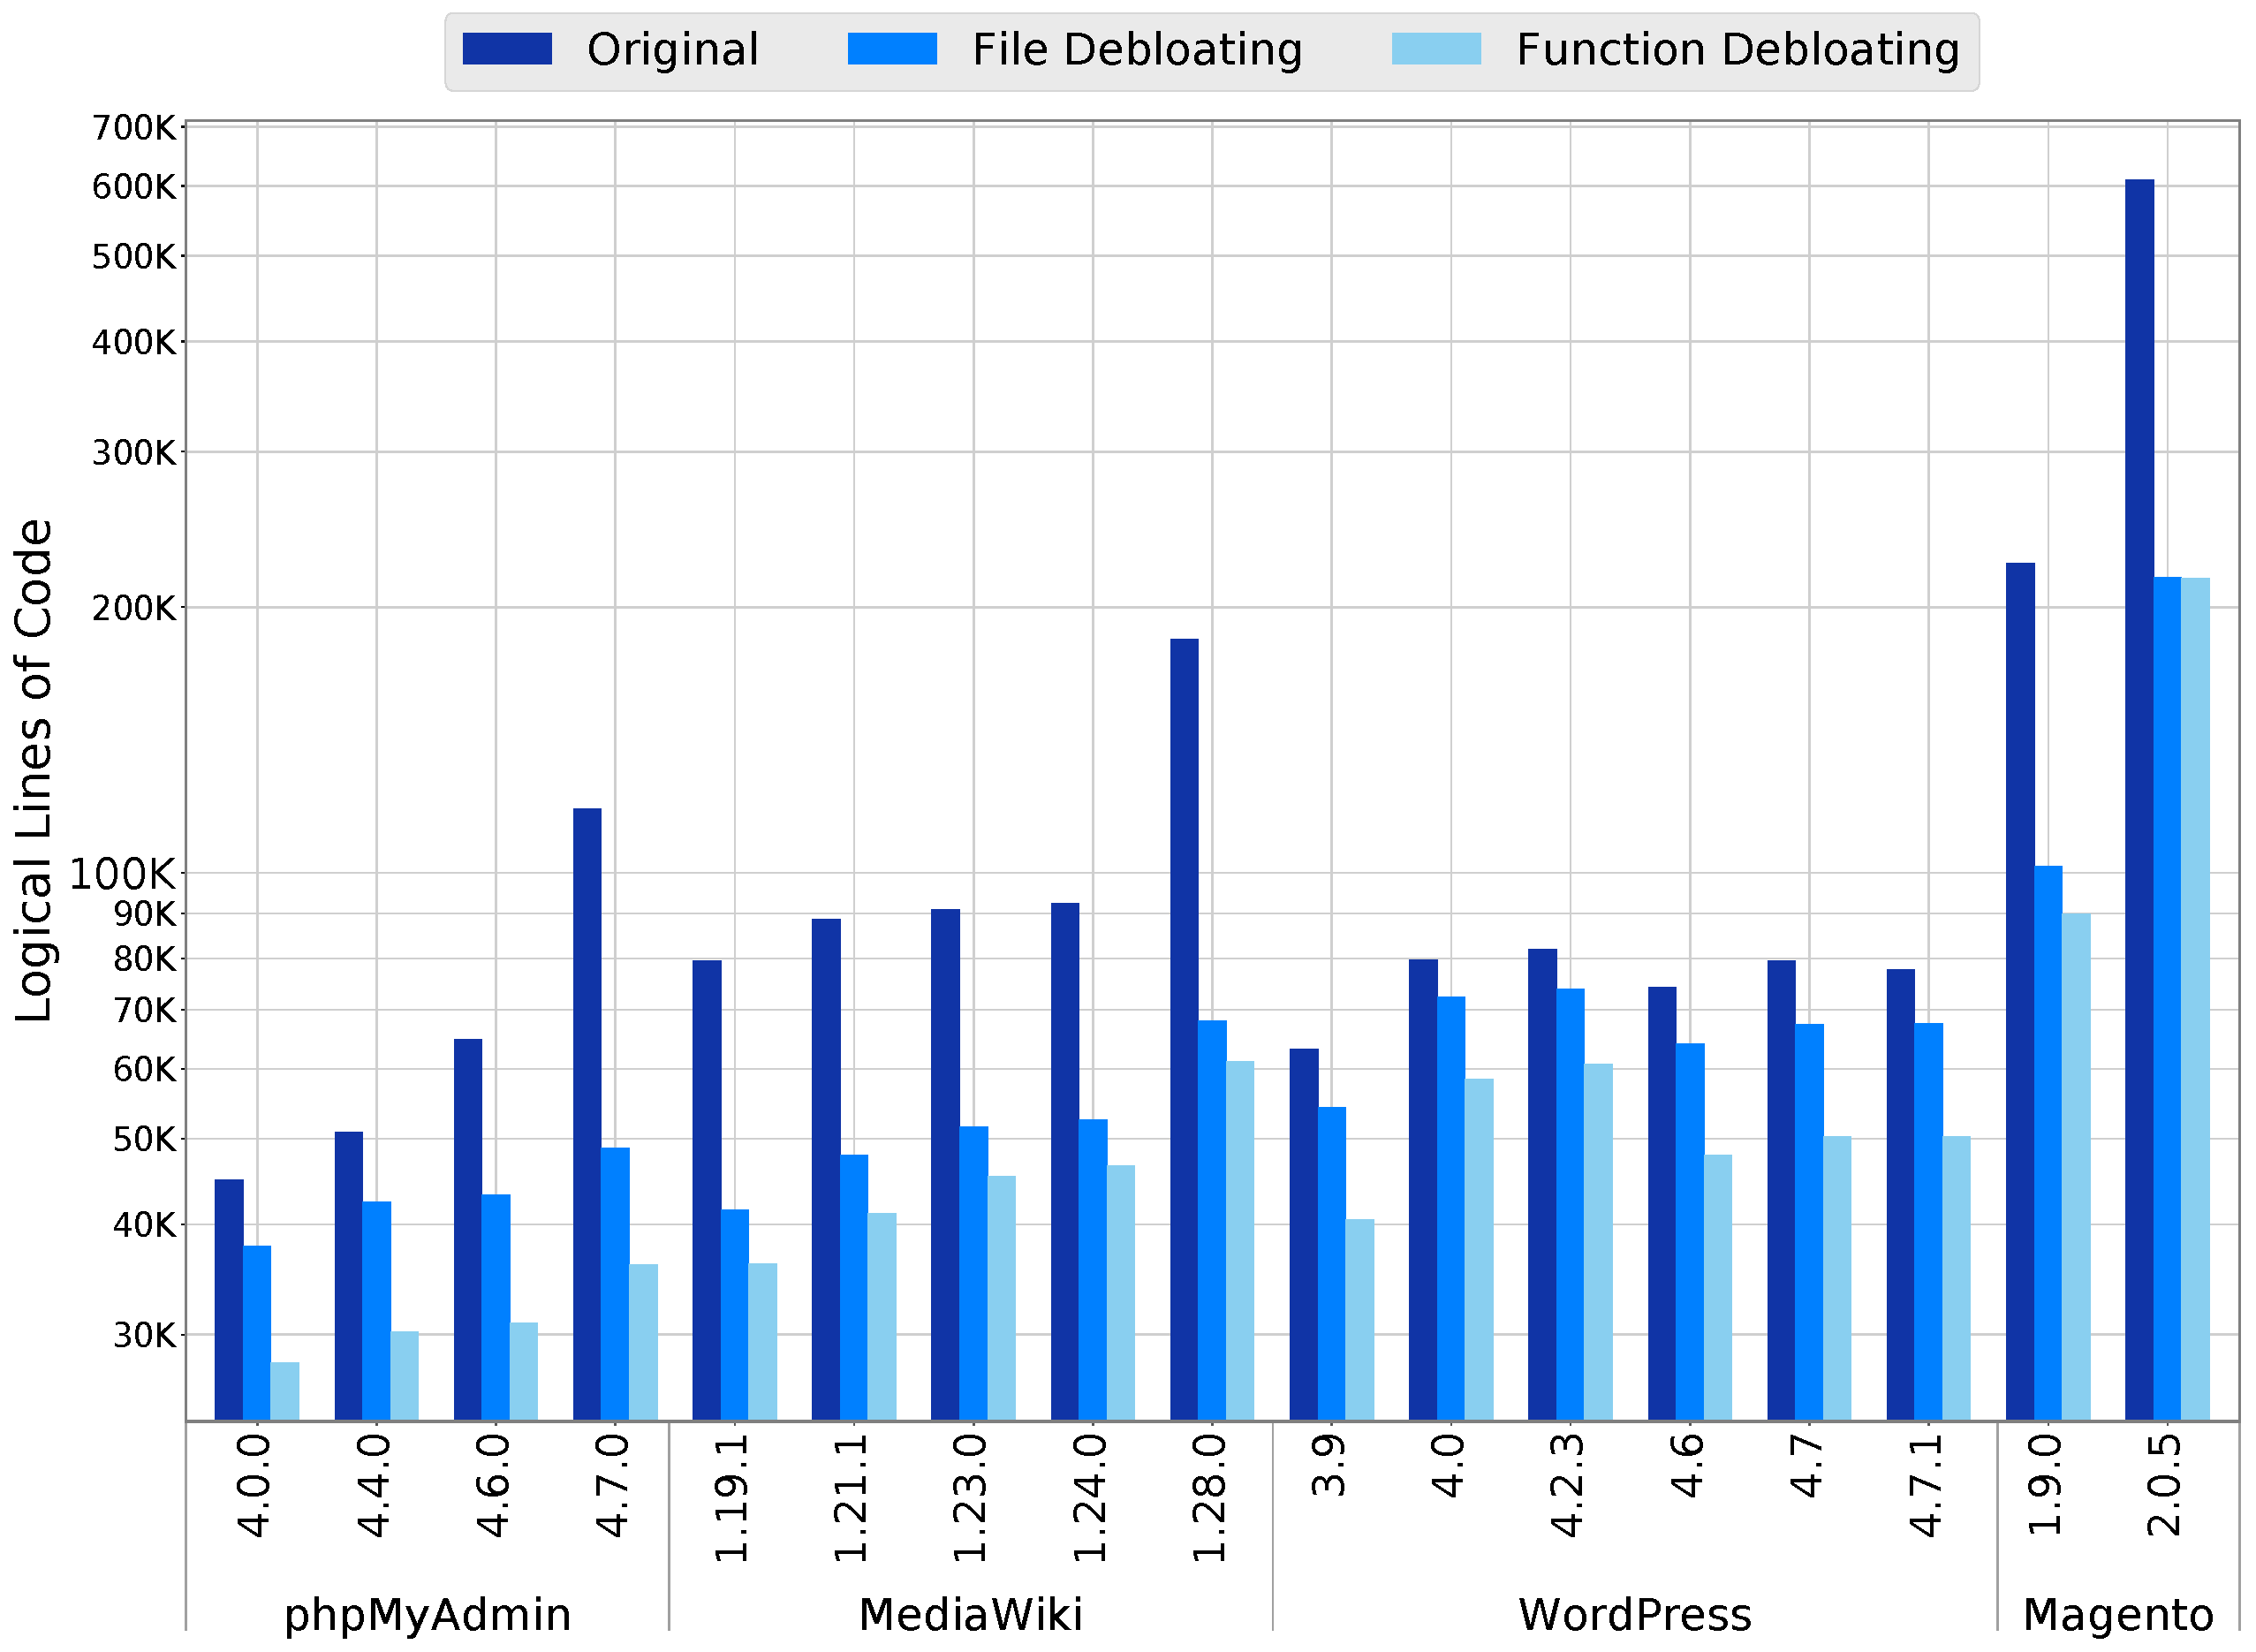
\includegraphics[width=\linewidth]{figures/lim/lloc.pdf}
  \caption{Logical Lines of Code before and after debloating}
  \label{fig:lloc}
\end{figure}


\paragraph{File-level debloating.}
Overall, file-level debloating, the most conservative of the two evaluated
debloating strategies, is already effective in reducing the number of LLOC with an average of 33.1\% reduction.
The minimum observed in our experiment is 9.2\% for WordPress
v.4.0 and a maximum of 64.5\% for Magento v.2.0.5. For Magento,
this reduction represents a removal of 393K lines of code.
This number is a clear sign that large web applications encompass many
different features that may not be used by all users and therefore result
in bloated applications with an unnecessarily large attack surface. At the same time, it is worthwhile repeating that all debloating results presented in this section are conditional to how web applications are used. Therefore, these large levels of debloating cannot be guaranteed for all possible deployments of web applications. We discuss this issue in Section~\ref{sec:limitations}.

\paragraph{Function-level debloating.}
On average, function-level debloating is able to remove 46.8\% of lines of code.
For both Magento and MediaWiki, it can remove up to
7\% more code over file-level debloating. For phpMyAdmin and WordPress, we observe an
increase of debloating capability of up to 24\%. This
larger reduction (compared to MediaWiki and Magento) is mainly due to
the differences in software development practices.

Compared to the other
tested applications, phpMyAdmin and WordPress are more monolithic with a smaller number of large
source-code files. Since file-level debloating only removes files when none
of their functions were executed, the monolithic nature of these two applications resists
this kind of coarse-level debloating. Contrastingly, Magento and MediaWiki
are developed in a much more modular fashion (many small files each responsible
for a small number of well-defined tasks) and therefore lend themselves better to file-level
debloating. The more fine-grained, function-level debloating bypasses this
issue and can therefore reduce the attack surface of a web application,
even for more monolithic web applications.


\subsubsection{Cyclomatic complexity}
\label{subsubsec:cyclomatic-complexity}
Next, we look at the evolution of cyclomatic complexity (CC). CC is defined as
the number of linearly independent paths through the code of
an application~\cite{mccabe1976complexity}. A high CC for a
single class implies complicated code that is difficult to
debug and maintain~\cite{gill1991cyclomatic} and therefore
more prone to contain vulnerabilities when compared to code with low
CC~\cite{shin2008empirical,kurmus2013attack}.

\begin{figure}[t]
  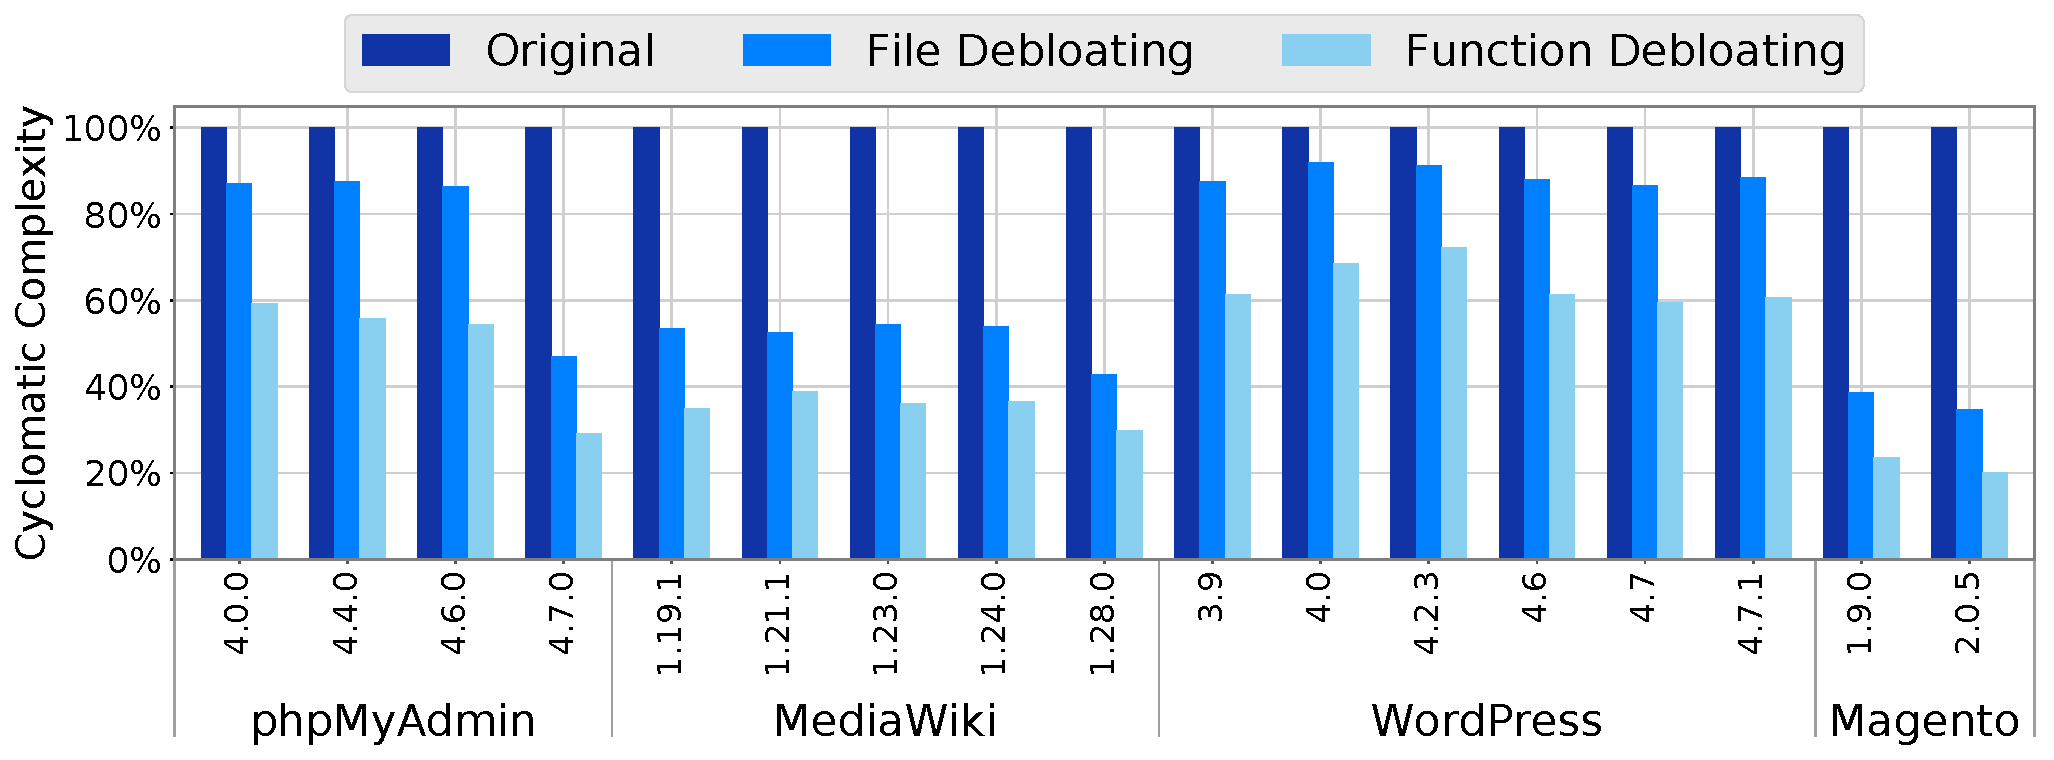
\includegraphics[width=\linewidth]{figures/lim/cc_over_loc.pdf}
  \caption{Evolution of cyclomatic complexity before and after debloating}
  \label{fig:ccoverloc}
\end{figure}

Figure~\ref{fig:ccoverloc} reports on the evolution of the overall CC for
each tested version in our experiment. File-level debloating decreases
CC between 5.9\% to 74.3\% with an average of 32.5\%.
Function-level debloating decreases the program complexity between 23.8\% and 80.2\% with an average of 50.3\%.
These statistics demonstrate that
debloating can remove complex instructions and execution paths in addition to
simple ones. Moreover, the difference between file-level and function-level
debloating shows that code removal through function-level debloating is much
more suited to all kinds of web applications as shown earlier through LLOC
reduction achieved via function-level debloating.


\begin{table}[t]
\caption{Number of CVEs removed after application debloating}
\centering
\scalebox{0.72}{
\begin{tabular}{|c|l|l|l|l|l|}
\hline
\multicolumn{1}{|l|}{\textbf{Application}} & \textbf{Strategy}   & \multicolumn{2}{l|}{\begin{tabular}[c]{@{}l@{}}\textbf{Total}\\ \textbf{Removed CVEs}\end{tabular}} & \multicolumn{2}{l|}{\begin{tabular}[c]{@{}l@{}}\textbf{Removed}\\ \textbf{Exploitable CVEs}\end{tabular}} \\ \hline
\multirow{2}{*}{phpMyAdmin}       & File Debloating     & 4/20                                    & 20 \%                                   & 3/19                                      & 15.7 \%                                     \\ \cline{2-6}
                                  & Function Debloating & 12/20                                   & 60 \%                                   & 11/19                                     & 57.8 \%                                     \\ \hline
\multirow{2}{*}{MediaWiki}        & File Debloating     & 8/21                                    & 38 \%                                   & 3/16                                      & 18.7 \%                                     \\ \cline{2-6}
                                  & Function Debloating & 10/21                                   & 47.6 \%                                 & 5/16                                      & 31.2 \%                                     \\ \hline
\multirow{2}{*}{WordPress}        & File Debloating     & 0/20                                    & 0 \%                                    & 0/20                                      & 0 \%                                        \\ \cline{2-6}
                                  & Function Debloating & 2/20                                    & 10 \%                                   & 2/20                                      & 10 \%                                       \\ \hline
\multirow{2}{*}{Magento}          & File Debloating     & 1/8                                     & 12.5 \%                                 & 1/8                                       & 12.5 \%                                     \\ \cline{2-6}
                                  & Function Debloating & 3/8                                     & 37.5 \%                                 & 3/8                                       & 37.5 \%                                     \\ \hline
\end{tabular}
}
\label{table:debloatingcvesresults}
\end{table}

\subsection{Analysis of CVEs}
In this section, we investigate the number of removed CVEs after debloating
along with the effects of debloating on different vulnerability categories.

\subsubsection{CVE reduction after debloating}
\label{sec:cve_reduction}
One practical way to measure the security benefits of debloating web
applications is to study the effects of debloating on known historical
vulnerabilities. If vulnerabilities were part of the core functionality of the
program, the evaluated debloating strategies will not be able to remove the
code associated with them. However, if some vulnerabilities reside in parts
of a web application that are not commonly used, the process of debloating
can effectively remove them.


Table~\ref{table:debloatingcvesresults} compares the effectiveness of
debloating strategies by listing the fractions of removed CVEs. We consider
a vulnerability to have been successfully removed if all the lines of code
and functions associated with that vulnerability were removed during the
stage of debloating. This is a conservative approach as one modification
performed on a single line could thwart a complete attack. As such, the
numbers we report in this section can be interpreted as lower bounds of
the actual number of removed CVEs.


In terms of configuration, we selected the default one for each application.
However, certain vulnerabilities may not be exploitable under this configuration.
For example, there exists 5 CVEs in our dataset for MediaWiki which require file upload functionality to be enabled. Since this option is disabled by default, we make an explicit distinction in the table.
``Total Removed CVEs'' is the total number of CVEs removed by debloating regardless of whether the vulnerable code is enabled or disabled through a configuration option. ``Removed Exploitable CVEs'' reports on the CVEs that are reachable under default configurations of target web applications.
%Certain vulnerabilities may not be exploited under the default configuration of target applications. For example there exists 5 CVEs in our dataset for MediaWiki which require file upload functionality to be enabled. Since this option is disabled by default,
%we ran our tests with and without this feature enabled and reported both numbers.
%``Total Removed CVEs`` is the the total number of CVEs removed by debloating regardless of vulnerable code being enabled through configuration settings and ``Removed Exploitable CVEs'' reports on the CVEs that are reachable under default configurations of target web applications.

On average, we discovered that up to 38~\% of vulnerabilities are removed by
file debloating whereas 10-60~\% are removed by function debloating. As
shown in Table~\ref{table:debloatingcvesresults}, function-level debloating
can triple (in the case of phpMyAdmin and Magento) the number of removed CVEs, compared to file-level debloating. This
behavior can be generalized to web applications that do not have CVE
information and demonstrates that the reduction of a web application's
LLOC (Section~\ref{subsubsec:lloc}) and its cyclomatic complexity
(Section~\ref{subsubsec:cyclomatic-complexity}) translates to a reduction
of concrete vulnerabilities. Wordpress is a clear negative outlier with only
10\% CVE reduction, even through the more flexible function-debloating
strategy. As mentioned earlier, WordPress is a relatively monolithic
application and most of our mapped CVEs are located in core WordPress code (e.g.,
Authentication, CSRF tokens, and post/comment-related actions) which cannot
be removed by our debloating framework.








\begin{figure}[t]
  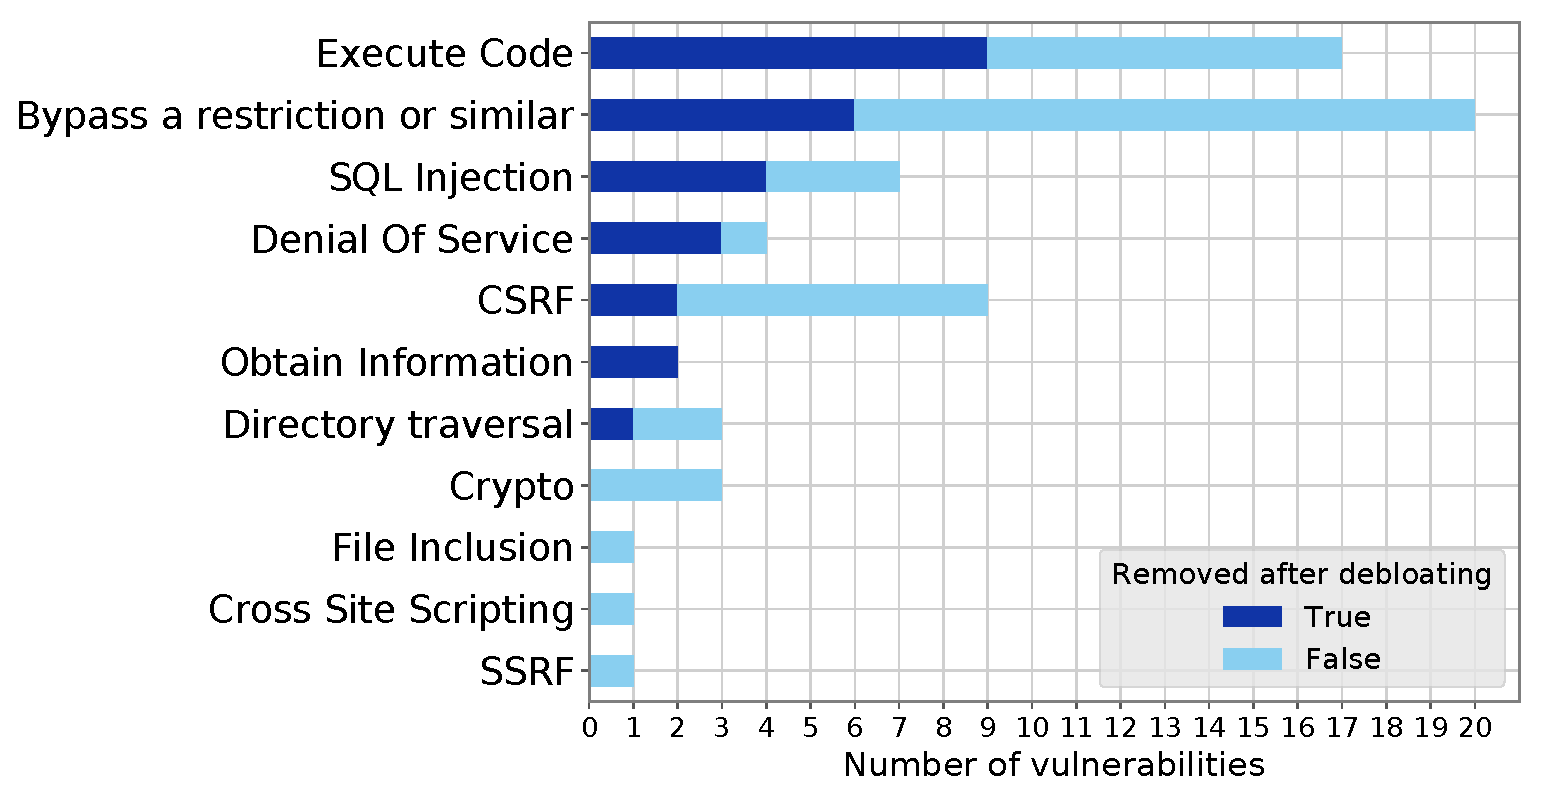
\includegraphics[width=\linewidth]{figures/lim/vuln_per_category.pdf}
  \caption{Vulnerability Categories}
  \label{fig:vulnpercat}
\end{figure}

\subsubsection{Types of CVEs in analyzed web applications}

Even though our results demonstrate the ability to remove vulnerabilities
from web applications through the use of debloating, one may wonder
whether debloating is better suited for some types of vulnerabilities over
others. Figure~\ref{fig:vulnpercat} provides details on the categories of
the CVEs we removed through debloating.


One can observe that for certain classes of vulnerabilities, such as,
Denial-of-Service attacks and Information-Revealing vulnerabilities,
debloating can almost completely remove them.
For others, such as, restriction bypassing, command execution, and
SQL injection, debloating can substantially reduce them.
Our interpretation of these findings has to do with the maturity of
the evaluated web applications. Specifically, all four web applications
have been available for a long period of time, allowing many shallow
vulnerabilities to have already been discovered and corrected. The remaining
vulnerabilities are likely to be situated in parts of a web application that
are less commonly exercised. For example, the code-execution vulnerabilities
that can be removed for phpMyAdmin are inside very specific features, such as,
the ability to export PHP arrays (CVE-2016-6609), the support of the
ZIP extension while importing data (CVE-2016-6633), and the abilities
to copy table definitions (CVE-2013-3238) and perform Regex search and replace over table columns
(CVE-2016-5734).

\begin{table*}[t]
\caption{Statistics on the external packages included in web applications and the effects of debloating in terms of reducing their LLOC.}
\centering
\scalebox{0.5}{
\begin{tabular}{c|c|c|c|c|c|c|c|c|c|}
\cline{2-10}
 & \multicolumn{3}{c|}{\textbf{Before debloating}} & \multicolumn{6}{c|}{\textbf{After function-level debloating}} \\ \hline
\multicolumn{1}{|c|}{\multirow{2}{*}{\textbf{Application}}} & \multirow{2}{*}{\begin{tabular}[c]{@{}c@{}}\# \textit{lines in main}\\\textit{application}\end{tabular}} & \multirow{2}{*}{\begin{tabular}[c]{@{}c@{}}\textit{\# lines in}\\\textit{packages}\end{tabular}} & \multirow{2}{*}{\textit{\# packages}} & \multirow{2}{*}{\begin{tabular}[c]{@{}c@{}}\textit{\# lines in main}\\ \textit{application}\end{tabular}} & \multirow{2}{*}{\begin{tabular}[c]{@{}c@{}}\textit{\# lines in}\\\textit{packages}\end{tabular}} & \multirow{2}{*}{\begin{tabular}[c]{@{}c@{}}\textit{\# packages}\\\textit{completely}\\\textit{removed}\end{tabular}} & \multicolumn{3}{c|}{\begin{tabular}[c]{@{}c@{}}\textit{\# packages where a given \%}\\\textit{lines were removed}\end{tabular}} \\ \cline{8-10}
\multicolumn{1}{|c|}{} &  &  &  &  &  &  & \textgreater{}\textit{70\%} & \begin{tabular}[c]{@{}c@{}}\textless{}\textit{70\% and}\\ \textgreater{}\textit{30\%}\end{tabular} & \textless{}\textit{30\%}\\ \hline
\multicolumn{1}{|c|}{phpMyAdmin 4.7.0} & 35,739  & 82,604  & 45 & 26,377 (-26.2\%)  & 9,653 (-88.3\%)  & 38 (84.4\%) & 2 & 1  & 4  \\ \hline
\multicolumn{1}{|c|}{MediaWiki 1.28.0} & 133,019 & 50,898  & 40 & 54,827 (-58.8\%)  & 6,285 (-87.7\%)  & 24 (60.0\%) & 2 & 2  & 12 \\ \hline
\multicolumn{1}{|c|}{Magento 2.0.5}    & 396,448 & 212,906 & 71 & 181,696 (-54.2\%) & 34,038 (-84.0\%) & 58 (81.7\%) & 6 & 5  & 2  \\ \hline
\end{tabular}
}
\label{table:numberofpackages}
\end{table*}


Contrastingly, the three cryptography-related vulnerabilities we analyzed are
still present in the debloated versions of web applications. One of the CVEs
related to this category is about a flaw in the cookie encryption algorithm in
phpMyAdmin (CVE-2016-6606). Since every page interacts with user
cookies to, at the very least, verify them, vulnerable code cannot be
removed. Another vulnerability in this category relates to an insecure random
number generator used in cryptographic operations by Magento (CVE-2016-6485).
This vulnerability exists in a constructor of the main encryption
classes which is widely used throughout the application. When considered
together, these findings suggest that cryptography-related vulnerabilities
are a core part of web applications and thus unlikely to be removed through
the process of debloating.




\subsection{External packages}
\label{subsec:external}

\subsubsection{Quantifying the bloat from external packages}

In our testbed, phpMyAdmin v.4.7.0, MediaWiki v.1.28.0 and Magento v.2.0.5 rely
on external dependencies that can be downloaded via Composer (WordPress does not rely on external packages). As described in
Section~\ref{sec:background}, Composer is a package manager for PHP (similar
to the NPM manager for NodeJS applications) which allows web applications
to specify which external packages they rely on and have these packages be
tracked and updated.

As we briefly discussed in Section~\ref{subsubsec:lloc}, the number of LLOC of
these three specific versions dramatically
increases (compared to prior versions) because of this dependency on external
packages. Table~\ref{table:numberofpackages} provides statistics on the
number of packages pulled by these applications and how much bloat they
provide against our usage profiles.


First, one can observe that external packages introduce a large amount of
unused code. For all three debloated applications, more than 84\% of their code
was removed from them. This means that the attack surface is unnecessarily
large through the dependency on external packages. The number of removed
lines from external packages for Magento is particularly noteworthy with
more than 178,000 lines of code removed. Moreover, the number of packages
that can be completely removed is also quite large: 84\% for phpMyAdmin,
60\% for MediaWiki and 81\% for Magento. This confirms that most packages
are unnecessary for the usage profiles that we recorded. Finally, focusing
exclusively on the lines of code, phpMyAdmin is the only application where
external packages have more lines than the main application. However, after
debloating, this relationship is reversed with the codebase of phpMyAdmin
being three times the size of the introduced external packages.


Despite the advantages of using package managers (e.g., the ability to track
dependencies and update vulnerable libraries without the need to update
the main application), our findings show that these advantages come at a
considerable cost in terms of unnecessarily expanding the attack surface of
a web application with code that is seldomly executed. As such, developers
must take special care to include the bare minimum of external packages,
knowing the unwanted side-effects that each external package brings.

\subsubsection{Removing POI gadgets}

\paragraph{What are POI gadgets?}
Property Oriented Programing (POP) is an exploitation technique
in PHP which works similarly to Return Oriented Programming
(ROP)~\cite{shacham2007geometry} and is used to exploit PHP Object Injection
(POI) vulnerabilities~\cite{POI}. In this technique, the attacker creates
exploit gadgets from available code in the applications. By chaining
multiple gadgets within the application, an attacker can usually run
arbitrary code, write to arbitrary files, or interact with a database. Dahse
et al. have studied the automatic generation of such gadget chains for PHP
applications~\cite{Dahse:2014:CRA:2660267.2660363}.

\paragraph{PHP unsafe deserialization.}
The PHP language gives developers the ability to serialize arbitrary objects in
order to store them as text, or transfer them over the network. Deserialization
reverses this process, generating PHP objects from serialized data. This
mechanism can be abused by an attacker to load specific classes in the
application and build a gadget chain. Practical examples of this vulnerability
are when \texttt{unserialize} is called on a database field or value of a
field within a cookie that can be manipulated by the users.

Historically, this attack was very difficult to successfully execute. Attackers
could only build gadgets with the classes that were present in the context of
the vulnerable file. They needed insights into how the application was built
in order to know which classes could be abused for gadgets. However, starting
from PHP 5, the \texttt{\_\_autoload()} magic function~\cite{PHPAutoload}
was introduced and unintentionally made exploitation of deserialization
vulnerabilities easier. This new loading feature was beneficial for PHP
developers who did not have to manually include all the files they wanted to
use at the very top of each of their PHP files. It also helped the adoption
of package managers like Composer, as any external dependency could be easily
called from anywhere in the application. The downside of this new function
was that it also allowed attackers to instantiate any PHP class across the
entire application thereby enabling the easier construction of gadget chains.

In order to build a chain, attackers use these so-called ``magic''
functions~\cite{PHPWakeup} that form the basis of their gadget chain. One of
the functions that is widely used in POI exploits is the \textit{destruct}
function. In Section~\ref{subsec:coverage}, we detailed the challenges in
getting complete coverage of destructors in our tested applications. Accurate
coverage of destructors also allows us to precisely analyze the impact of
debloating on gadget creation.




\paragraph{Can debloating remove gadgets from external packages?}

Given the increased footprint of web applications due to their reliance
on package managers and external dependencies, one may wonder about the
possibility of abuse of these packages for the creation of gadgets. To
measure the effect of debloating on Property-Oriented-Programming (POP)
gadgets, we utilized the PHPGGC~\cite{PHPGGC} library. PHPGGC (which stands
for PHP Generic Gadget Chains) contains a list of known gadgets in popular
PHP packages such as Doctrine, Symfony, Laravel, Yii and ZendFramework. When
a vulnerable PHP application includes any of the packages listed in PHPGGC,
the attackers can generate gadget chains to achieve RCE, arbitrary file
writes, and SQL injections.

We analyzed the available gadget chains in PHPGGC and
checked whether any of our tested PHP applications included these
chains. Table~\ref{table:knowngadgets} summarizes the presence of each gadget
and whether debloating removes them or not. WordPress is not included in this table because it does not rely on external packages.
This does not make WordPress immune to POI attacks, but universally known gadget chains in popular external packages can not be used to exploit WordPress.
%Note that while packages such as Symfony are used across our tested web applications, the specific component required to create gadget chains was not pulled by any of tested applications. Such cases are omitted from our results.
For the affected applications, file-level debloating removes 4/6 gadgets while function debloating removes
6/6 available gadget chains. This again demonstrates the power of debloating
which can not only remove some fraction of vulnerabilities but also make
the exploitation of the remaining ones harder by removing the gadgets that
attackers could abuse during a POI attack.


\begin{table}[]
  \centering
  \caption{List of packages with known POP gadget chains}
\scalebox{0.9}{
\begin{tabular}{|l|l|c|c|}
\hline
\multirow{2}{*}{\textbf{Application}}      & \multirow{2}{*}{\textbf{Package}} & \multicolumn{2}{l|}{\begin{tabular}[c]{c@{}c@{}}\textbf{Removed by}\\\textbf{Debloating}\end{tabular}} \\ \cline{3-4}
    &    & \textit{File}     &  \textit{Function}                                     \\ \hline
\multirow{2}{*}{phpMyAdmin 4.7.0} & Doctrine                 & \faCheck                                         & \faCheck                                            \\ \cline{2-4}
                                  & Guzzle                   & \faCheck                                         & \faCheck                                            \\ \hline
MediaWiki 1.28.0                  & Monolog                  & \faCheck                                         & \faCheck                                            \\ \hline
\multirow{3}{*}{Magento 2.0.5}    & Doctrine                 & \faCheck                                         & \faCheck                                            \\ \cline{2-4}
                                  & Monolog                  & \faTimes                                         & \faCheck                                            \\ \cline{2-4}
                                  & Zendframework            & \faTimes                                         & \faCheck                                            \\ \hline
\end{tabular}}
\label{table:knowngadgets}
\end{table}


\subsubsection{Utilizing development packages in production}
During our analysis of external packages, we identified yet another source
of bloat in new versions of web applications. When declaring external
dependencies through Composer, two options are available: ``require'' and
``require-dev''. The first option indicates packages that are mandatory for
the application to run properly. The second lists packages that should only be
used in development environments, such as, packages providing support for unit
testing, performance analysis, and profiling. We discovered that applications
downloaded from official websites often include these development packages. As
such, when these packages are used to deploy web applications in production
mode, they will contain unnecessary development libraries. This does not
only increase the attack surface by having unnecessary code bloating the
application, but can also lead to exploitation for misconfigured applications.

CVE-2017-9841 presents one example of such a
vulnerability~\cite{phpunitVulnerability}. Specifically, this CVE refers
to an RCE attack in specific versions of the PHPUnit library, which is
a popular unit testing library for PHP. By default, Composer places all
external packages under ``vendor'' directory. If this specific directory
happens to be accessible through a misconfiguration of the server, PHPUnit
files are then accessible and can be exploited to conduct an RCE attack.

The four web applications that we evaluated for this study, present
different behaviors with respect to development packages. WordPress does not rely on external packages downloaded through Composer.
MediaWiki never
included development packages in its releases. phpMyAdmin had them in version
4.7.0 but stopped including them in version 4.8.3 (the latest at the time of
writing). Magento started including them from version 2.0 and still includes
them today. We have reached out to Magento and informed them about this issue.


\subsection{Qualitative analysis of the removed code}
\label{subsec:qualitative}

In the previous sections, we analyzed the effects of debloating on the source code of applications from a software-engineering perspective (i.e., LLOC and Cyclomatic Complexity reduction) as well as from a security standpoint (i.e., number of CVEs and gadgets removed). At the same time, one may wonder what exactly was removed from each application during the process of debloating.



Given that thousands of files were removed, manually analyzing each file does not scale. As such, we turn to NLP techniques that allow us to cluster the removed files together and provide us with hints about the nature of each cluster. Specifically, we use the k-means clustering algorithm based on text vectors extracted from removed file names and file paths. Each file path includes directories that indicate which library or package, the file belongs to. For most modern web applications, this allows for a reasonable separation of files across different application plugins and modules.
To end up with meaningful clusters, we tuned TFIDF vectorizer parameters along with the number of k-means clusters. We used the TFIDF maximum frequency limit to ignore common terms appearing in more than 50\% of the files. Depending on the size and modularity of the application, 10 to 20 clusters yielded the most instructive grouping of files.

Table~\ref{tab:removed_files_categories} shows the categories of the three largest removed clusters from each web application. Across all four applications, we observe the removal of source code related to external packages (e.g., Symfony for phpMyAdmin, Elastica for MediaWiki, and Zendframework1 for Magento), followed by localization/theme files (e.g., twentyfourteen theme for WordPress), and unused database drivers. We provide more application-specific details of removed features in the next paragraphs.

\begin{table}[t]
  \caption{Features and external packages with the most removed files after file debloating (removed features are marked in italic). Entries marked with $\ast$ are packages that are indirectly pulled by other ``require-dev'' packages (not used by core application) for the purpose of test coverage reporting and coding standard enforcement.}
  \label{tab:removed_files_categories}
  \centering
\scalebox{0.75}{
\begin{tabular}{|l|l|}
\hline
\textbf{Applications} & \textbf{Features/Packages with most files removed} \\ \hline
                           & 1) Guzzle~\cite{guzzle}: ``Generating API HTTP response'' *  \\
\textit{phpMyAdmin 4.7.0}  & 2) Symfony~\cite{Symfony}: ``Parsing configuration files'' * \\
                           & 3) PHP\_CodeSniffer~\cite{PHP_CodeSniffer}: ``Enforcing coding standards'' * \\ \hline
                           & 1) \textit{Messages \& Languages} \\
\textit{MediaWiki 1.28.0}  & 2) Less.php~\cite{less.php}: ``Generating CSS code'' \\
		                       & 3) Elastica~\cite{elastica}: ``Elastic search interface used by\\ & extensions'' \\ \hline
                           & 1) Twentyfourteen theme~\cite{twentyfourteen_theme} \\
\textit{WordPress 4.7.1}	 & 2) Twentytwelve theme~\cite{twentytwelve_theme} \\
		                       & 3-4) Also theme related \\
		                       & 5) \textit{Multi-site administration} \\ \hline
	                         & 1) Zendframework1~\cite{zendframework1}: ``Generating web pages and\\
\textit{Magento 2.0.5}     & database operations'' \\
		                       & 2) \textit{Sales, Orders \& Credit Memo} \\
		                       & 3) \textit{Internal framework filters \& Views} \\ \hline
\end{tabular}
}
\end{table}

\vspace{0.5ex}
\noindent\textbf{phpMyAdmin's} removed features include the uploading of plugins, GIS visualizations, and unused file formats used in import/export (such as, Dia, EPS, PDF, SVG, and ZIP). In addition, debloating removed unused plugins and external packages which make up the top 3 features removed from this web application as shown in Table~\ref{tab:removed_files_categories}. phpMyAdmin version 4.6.0 and 4.7.0 include unit tests which are also removed by our system. The LLOC for the removed test files is less than 2\% of the whole code base of the application.

\vspace{0.5ex}
\noindent\textbf{MediaWiki} provides an API to interact with the wiki which is separate from the regular web interface that users interact with. Most actions within this API, including queries, file upload, and non-default output formats for this API were removed. Top categories of removed files consist of localization of messages and language files in addition to external dependencies (Lines 2 and 3) as listed in Table~\ref{tab:removed_files_categories}. The debloating process also removes file-upload modules which are disabled, by default, in MediaWiki. It is important to note that even if a module is ``disabled,'' the code still resides on the server and could be abused by specific types of attacks. For example, in a recent attack against a WordPress plugin, the vulnerability could be exploited even if that plugin was disabled~\cite{wordpressPlugin}. Debloating \textit{removes} the source code of disabled and unused features and therefore does not suffer from this type of attack.
Finally, the process of debloating, removed unused extensions of Mediawiki (e.g., citation, input box, pdf handler, poem and syntax highlighting). Mediawiki 1.19.1 and 1.28.0 include unit tests, and they measure less than 1.5\% of LLOC in the whole code base of their respective versions.

\vspace{0.5ex}
\noindent\textbf{WordPress} takes a slightly different approach where the core functionality is concentrated in a relatively small number of large PHP files. The removed features of WordPress include installation files, unused modules (FTP, multi-site, user registration), disabled themes and update files (note that we could not exercise update files during our tests because this would change the version of the evaluated web application and create inconsistencies in our analysis of removed CVEs). In terms of testing, the installation files that we obtained from the WordPress website do not contain any unit tests.

%Interestingly, WordPress contains less code bloat. That is because most of the functionality within this application is exercised by tutorials and other tests, and this is not the result of more comprehensive tutorials. As WordPress has a monolithic nature that does not rely on external dependencies (the main source of bloat), the application does not include unnecessary features that only a subset of users would use. WordPress offloads these specific requirements to plugins. For instance, importing data into WordPress which is available in other studied software requires a separate plugin. As a result, most of the existing modules in vanilla WordPress would be exercised throughout the dynamic analysis tests with the exception of few that are mentioned above. This also affects the mapped CVEs for core WordPress in that the CVEs mostly target core functionality (e.g., Authentication, CSRF tokens and post and comment related actions).

\vspace{0.5ex}
\noindent\textbf{Magento} consists of both external packages and internal modules. We observed that various internal modules were removed, including an XML API for mobile, wishlists, ratings, and specific payment modules (such as, Paypal). Since many packages and internal modules include the terms ``sales,'' ``orders,'' and ``tax,'' these individual files across multiple modules were clustered into the same category by k-means. Finally, Magento 1.9.0 does not include unit tests while the test files included in Magento 2.0.5 and its external packages measure up to 15\% of its code base. For Magento 2.0.5, Zendframework1 which is an external dependency has most of its files removed by debloating.

%\begin{table}[]
%  \caption{Top file categories removed by file debloating}
%  \label{tab:removed_files_categories}
%  \centering
%\scalebox{0.8}{
%\begin{tabular}{|l|}
%\hline
%\multicolumn{1}{|c|}{\textbf{Applications}}                        \\ \hline
%\multicolumn{1}{|l|}{\textbf{phpMyAdmin 4.7.0:}}                                                           \\ %\hline
%1) Guzzle 2) Symphony 3) squizlabs/php\_codesniffer                                              \\ \hline
%\multicolumn{1}{|l|}{\textbf{MediaWiki 1.28.0:}}                                                           \\ %\hline
%1) Messages \& Languages 2) oyejorge/less.php 3) ruflin/elastica                                 \\ \hline
%\multicolumn{1}{|l|}{\textbf{WordPress 4.7.1:}}                                                            \\ %\hline
%1) twentyfourteen theme 2) twentytwelve theme (3/4 are also themes) \\ 5) multi-site administration \\ \hline
%\multicolumn{1}{|l|}{\textbf{Magento 2.0.5:}}                                                              \\ %\hline
%1) Zendframework1 2) Sales, Orders \& Creditmemo \\ 3) Internal framework filters \& views          \\ \hline
%\end{tabular}
%}
%\end{table}



% Summary of removed features
%--- 4.0.0 ---
%
%Tracking, triggers, gis data, unused engines (berkeleydb, binlog, memory, myisam, ndbcluster)
%Unused encryption functions.
%Unused authentication mechanisms
%Uploading plugins
%Unused plugin transformations (Image inline or link, text to formats such as date)
%Export schema formats such as: Dia, Eps, Pdf, SVG and Visio.
%Zip extension.
%setup files.
%
%--- 4.6 ---
%
%Recaptcha plugin, Unused sql parser modules, test files.
%
%--- 4.7 ---
%
%External packages: doctrine/instantiator, gitonomy/gitlib, google/recaptcha, guzzle/guzzle, phpdocumentor, phpmyadmin/sql-parser, phpspec/prophecy, phpunit/php-code-coverage, timer, php-token-stream, %satooshi/php-coveralls, sebastian/comparator, sebastian/diff, sebastian/global-state, squizlabs/php\_codesniffer, symfony/cache, symfony/config, symfony/console, symfony/debug, symfony/event-dispatcher, %symfony/expression-language, symfony/filesystem, symfony/polyfill-mbstring, symfony/process, tecnickcom/tcpdf and webmozart.
%
%Mediawiki:
%
%--- 1.19.1 ---
%
%Unused APIs including: Formats such as JSON, PHP, XML, YAML, txt and raw. Action APIs: Authentication, Queries, Fileupload.
%Caching such as memcached, object file and resource file cache.
%Database drivers such as: MSSQL, Postgres, Oracle, Sqlite and db2.
%File repo
%Installation files.
%Media formats such as DjVu, GIF, PNG, SVG and XMP.
%Parser tools such as diff and hasher.
%Profiler and Tracer tools.
%Search modules for unused database drivers.
%Upload modules such as upload from URL, stash or upload in chunks.
%Unused language files and skins.
%Maintenance files such as benchmarks and clean up files.
%
%--- 1.21.1 ---
%
%Extensions such as citation, confirm edit, gadgets, image map, input box, interwiki, pdf handler, poem, rename user, syntax highlighting and title blacklists.
%
%--- 1.28.0 ---
%
%debug loggers, ``Exceptions!'', export to formats such as 7zip, bzip, dbzip2 and gzip.
%redis db modules, xml module, mail, rcfeed (machine readable recent changes)
%External packages: semver, cssjanus, php-jwt, james-heinrich/getid3, justinrainbow/json-schema, liuggio/statsd-php-client, monolog, kafka-php, oojs-ui, less.php, pear, pimple, ruflin/elastica, symfony/%process, vendor/wikimedia and zordius/lightncandy.
%
%Magento
%
%...
%
%WordPress:
%
%--- 3.9 ---
%
%FTP files, installation files, multisite modules, unused themes, sign up and new account activation, mail and trackback, cron and update file.
%
%--- 4.0 ---
%
%Export links from one blog to another. (opml)
%
%--- 4.7 ---
%
%pclzip library, fix corrupted database.

%\begin{table*}[]
%  \caption{Top file categories removed by file debloating}
%  \label{tab:removed_files_categories}
%  \centering
%\scalebox{0.69}{
%\begin{tabular}{|l|l|}
%\hline
%\textbf{Application}      & \textbf{Top file categories removed by debloating}                                                                                              \\ \hline
%phpMyAdmin 4.7.0 & 1) Guzzle 2) Symphony 3) squizlabs/php\_codesniffer 4) PHPUnit 5) phpsec/prophecy                                                                        \\ \hline
%MediaWiki 1.28.0 & 1) Messages \& Languages 2) oyejorge/less.php 3) ruflin/elastica 4) Installer \& Maintenance 5)james-heinrich/getid3                                     \\ \hline
%WordPress 4.7.1  & 1) twentyfourteen theme 2) twentytwelve theme 3) twentythirteen theme 4) twentytwelve theme 5) multi-site administration                                 \\ \hline
%Magento 2.0.5    & 1) Zendframework1 2) Sales, Orders \& Creditmemo 3) Internal framework filters \& views 4) Products, Sales, Shipping \& Tax 5) Widgets, Wishlists \& CMS \\ \hline
%\end{tabular}
%}
%\end{table*}
%}

\subsection{Testing debloated web applications against real exploits}
\label{section:metasploit}
To ensure the correct mapping of CVEs to source code and the ability of debloating to stop real attacks, we collected 4 exploits available in the Metasploit framework and augmented them with 4 POCs that we developed based on public bug-tracker records and vulnerability details. After verifying that we can successfully exploit the original versions of the evaluated web applications, we tested the same exploits on the debloated versions. Half of the previously successful exploits failed because the vulnerable code was removed during the process of debloating. Table~\ref{table:metasploit_vulns} lists the tested exploits against original and debloated applications.

As before, this demonstrates that while debloating is not a panacea against all possible issues, it can substantially improve the security of web applications. Finally, we present a demonstration of CVE-2016-4010 on Magento 2.0.5 in the following video: \url{https://vimeo.com/328225679}.



\begin{table}[]
  \centering
  \caption{Verifying exploitability of vulnerabilities by testing exploits against original \& debloated web applications}
  \label{table:metasploit_vulns}
  \scalebox{0.81}{
\begin{tabular}{|l|l|c|c|}
\hline
\multirow{2}{*}{\textbf{CVE}} & \multirow{2}{*}{\textbf{Target Software}} & \multicolumn{2}{c|}{\textbf{Exploit Successful?}} \\ \cline{3-4}
                     &                                  & \textbf{Original}           & \textbf{Debloated}          \\ \hline
CVE-2013-3238   & phpMyAdmin 4.0.0       & \faCheck & \faCheck                                                             \\ \hline
CVE-2016-5734   & phpMyAdmin 4.4.0       & \faCheck & \faTimes                                                             \\ \hline
CVE-2014-1610   & MediaWiki 1.21.1       & \faCheck & \faCheck                                                             \\ \hline
CVE-2017-0362   & MediaWiki 1.28.0       & \faCheck & \faTimes                                                             \\ \hline
CVE-2018-20714  & WordPress 3.9          & \faCheck & \faCheck                                                             \\ \hline
CVE-2015-5731   & WordPress 4.2.3        & \faCheck & \faCheck                                                             \\ \hline
CVE-2016-4010   & Magento 2.0.5          & \faCheck & \faTimes                                                             \\ \hline
CVE-2018-5301   & Magento 2.0.5          & \faCheck & \faTimes                                                             \\ \hline
\end{tabular}
}
\end{table}

\section{Performance analysis}
\label{subsection:performance}
It is known that code-coverage tools impose a non-negligible overhead on web applications~\cite{xdebug-performance1}. In this section, we report on the results of conducting all the Selenium tests with and without \texttt{XDebug} (our chosen PHP profiler) while measuring execution time, and recording server-side CPU usage and memory consumption. Table~\ref{table:performance} presents the overall results and Figure~\ref{fig:cpu} focuses on CPU consumption.

\begin{table}[]
  \centering
  \caption{Measurements of the execution time, the CPU and memory consumption for the tested web applications with XDebug and Code Coverage (CC) and without XDebug. The reported values for the CPU and memory correspond to the average for each application.}
  \label{table:performance}
\scalebox{0.7}{
\begin{tabular}{|c|c|c|c|c|}
\hline
\multicolumn{2}{|c|}{\textbf{Application}}              & \textbf{Execution (s)} & \textbf{CPU (\%)}       & \textbf{Memory (\%)}   \\ \hline
Magento     & \textit{Without XDebug} & 317           & 21.7           & 10.7          \\ \cline{2-5}
2.0.5       & \textit{With CC}    & 584 (x1.85)   & 56.9 (x2.62)   & 11.82 (x1.10) \\ \hline
MediaWiki   & \textit{Without XDebug} & 36            & 30.7           & 5.2           \\ \cline{2-5}
1.2.8       & \textit{With CC}    & 121 (x3.38)   & 79.3 (x2.58)   & 6.9 (x1.31)   \\ \hline
phpMyAdmin  & \textit{Without XDebug} & 102           & 3.7            & 5.7           \\ \cline{2-5}
4.7.0       & \textit{With CC}    & 116 (x1.14)   & 31.5 (x8.47)   & 5.6 (x0.97)   \\ \hline
WordPress   & \textit{Without XDebug} & 68            & 8.2            & 8.2           \\ \cline{2-5}
4.7.1       & \textit{With CC}    & 170 (x2.50)   & 42.6 (x5.22)   & 12.5 (x1.53)  \\ \hline
\end{tabular}
}
\end{table}

First, looking at the execution time, we can see that code coverage has a
varying impact on the tested web applications.
On one hand, phpMyAdmin is lightly affected with a 14\% increase.
On the other hand, the time it takes to run all tests for MediaWiki has
tripled.
For CPU consumption, the overhead is noticeable and all applications at
least double their use of resources when code coverage is active.
phpMyAdmin is exhibiting the biggest performance hit with a reported
average almost 9 times higher than the one from the base application.
Figure~\ref{fig:cpu} shows that all median values are higher for applications
with \texttt{XDebug} and most applications, at some point, require a second
core with values above 100\%. Finally, in terms of memory consumption,
the server-side code profiler incurs a relatively modest increase for most
applications. The worst overhead is observed when evaluating WordPress with
an increase of 4.3\% of the total device memory (16GB), i.e., an additional
700MB of RAM.

\begin{figure}[t]
  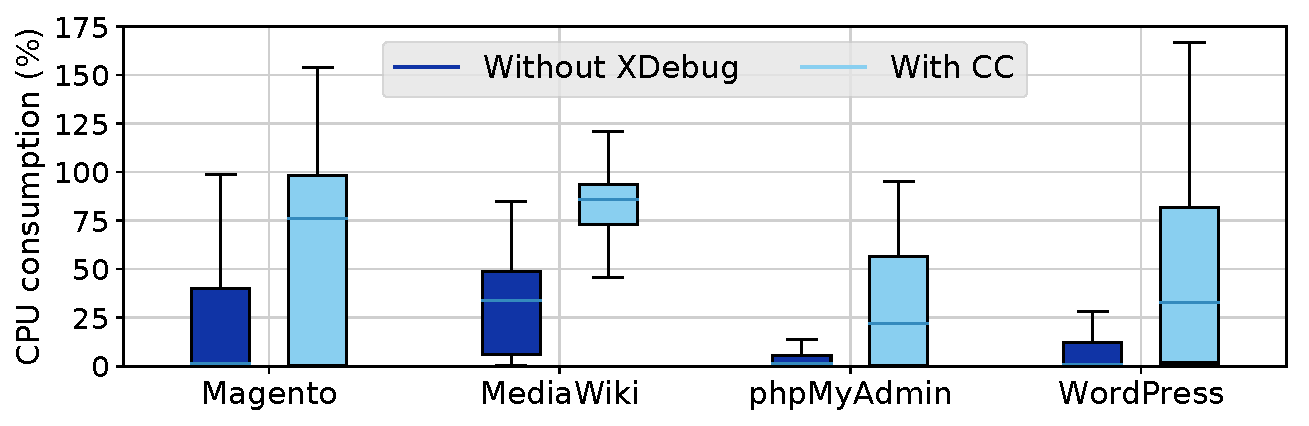
\includegraphics[width=\linewidth]{figures/lim/cpu.pdf}
  \caption{Measurement of the CPU consumption for the tested web
  applications. 100\% corresponds to the use of a single CPU core.}
  \label{fig:cpu}
\end{figure}

Even though our results show that the overall overhead is substantial, it is
important to note that this overhead is not the overhead of the debloated
web applications. Debloated web applications do not require code-coverage
statistics and will therefore execute in the exact same environment as
the original application (i.e., without \texttt{XDebug}). Depending on how
code-coverage information is obtained, this overhead may or may not be an
issue. For example, if the coverage is calculated in an offline fashion
where traces of application usage are replayed against a testing system,
this overhead will have no impact on the real production systems. To allow
for the online computation of code coverage (using real-time user traffic),
we need more optimized code profilers. For example, \texttt{XDebug} currently
overloads 43 opcodes to obtain line-level code-coverage information that
is more fine-grained than required by our debloating techniques and incurs
an unnecessary performance overhead~\cite{xdebug-performance2}. We leave
the development and evaluation of faster code profilers for future work.

\section{Limitations and future work}
\label{sec:limitations}
In this study, we set out to precisely quantify the security benefits of
debloating, when applied to web applications. Through a series of experiments,
we demonstrated that debloating web applications has a number of very
concrete advantages. We showed that debloating can, on average, decrease an
application's code base by removing hundreds of thousands of lines of code,
reduce its cyclomatic complexity by 30-50\% and remove code associated with
up to half of historical CVEs. Moreover, even for vulnerabilities that could
not be removed, debloating can remove gadgets that makes their exploitation
significantly harder. Next, we discuss some of the inherent and technical limitations of our approach and future direction.

\vspace{1ex}

\noindent\textbf{Lack of available exploits:} The number of exploits publicly available compared to the total number of registered CVEs is low. At the same time, the effort to study vulnerability reports, find the relevant patch or bug report, and track the actual vulnerability down to source code level takes a non-negligible amount of manual labor.
% Moreover, these public exploits usually favor certain types of vulnerabilities over others (e.g., favoring remote-command execution over XSS).
This lack of available exploits limits our ability to test the exploitability of vulnerabilities before debloating since certain vulnerabilities might only be exploitable under specific configurations.
For example the set of five file-upload-related vulnerabilities in our MediaWiki dataset (marked as gray in Table~\ref{table:listofallcves}) require access to file upload functionality which is disabled by default. A maintained set of automated, replayable exploits against popular web applications similar to ``BugBox'' introduced by Nilson et al. in 2013, could substantially help researchers at this step\cite{bugbox}.

To address this issue, we mapped the CVEs to features within those applications. This is done by studying the architecture of
target applications based on documentation within the code and available on their websites. We marked a CVE as unexploitable if the underlying feature is disabled by default, and online tutorials in our dataset do not
require users to enable that functionality. This limitation only applies to reported numbers on removed CVEs and does not affect our results on POI gadgets since their mere existence is enough for them to be used in gadget chains.

Our approach results in lower bounds for CVE removal since disabling modules through application configuration does not guarantee removal of all code paths that trigger those modules. Taking CVE-2019-6703 as an example, a vulnerability was discovered in the WordPress ``Total Donations'' plugin~\cite{wordpressPlugin} and disabling this plugin did not prevent attackers from invoking the vulnerable end point and running their exploits.

\vspace{1ex}
\noindent\textbf{Dynamic code coverage:}  Given our reliance on dynamic
code-coverage techniques, it is clear that the success of debloating a web application
is tightly related to its usage profile. Even though we constructed profiles
in a way that is reproducible and unbiased (i.e., by relying on external
popular tutorials, monkey testing, crawlers, and vulnerability scanners), we cannot claim that
real web users would not trigger code that was removed during the stage of
debloating, while they are interacting with a debloated web application.

More specifically, our modeled usage profiles do not cover all possible benign states of target web applications as we assume that users do not use all available features.
Our intuition behind debloating proves to be successful to a large degree since removing unnecessary features brings clear security improvements.
At the same time, our current usage model may not cover deep error states (e.g., logical errors in multi-stage form submissions, or the invalid structure of uploaded files).
As such, we intend to follow-up this work with crowd sourcing and user studies
to understand how administrators, developers, and regular users utilize the
evaluated web applications and whether their usage profiles would allow for
similar levels of debloating.

Due to nature of our approach, we can not take advantage of standard
static-analysis techniques, since we aim to remove the features that are
not useful for a given set of users, not those that are not reachable by
other code. Using static analysis would greatly overestimate the code that
needs to be maintained through the process of debloating and the resulting
web application would contain code (and therefore vulnerabilities) that is
not useful to all users. Going forward, we envision a hybrid approach where
dynamic analysis is used as a first step to identify the core features that
are useful for a specific set of users. These features can then be used as
a starting point for a follow-up static analysis phase to ensure that all
code related to these features is maintained when debloating a web application.

\vspace{1ex}
\noindent\textbf{Handling requests to removed code:}
A separate issue is that of handling requests to removed code. Our
current prototype utilizes assertions to log these requests so that we can
investigate why the corresponding server-side code was not captured by our
coverage profiler. When real users utilize debloated web applications,
one must decide how these failures (i.e., client-side requests requiring
server-side code that was removed) will be handled. Assuming that cleanly
exiting the application and showing an error to the user is not sufficient,
we need methods to authenticate the user's request, determine whether the
request is a benign one (and not a malicious request that aims to exploit
the debloated web application) and potentially re-introduce the removed
code. The client/server architecture of web applications lends itself well
to this model since the web server can decide to re-introduce debloated code
and handle the user's request, without any knowledge of this happening from
the side of the user. All of this, however, requires server-side systems
to introduce the code at the right time and for the appropriate users. We
leave the design of such systems for future work.

\vspace{1ex}
\noindent\textbf{Metrics to measure debloating effectiveness:}
In this paper, we use Cyclomatic Complexity (CC), Logical Lines of Code
(LLOC), reduction in historical CVEs, and POP gadget reduction as four metrics to measure the
effects of debloating on different web applications. However, not every line of code
contributes equally to a program's attack surface. For example, 15\% of removed
files from Magento 2.0.5 are test files for external packages and
the core of the application. Such code may not be directly exploitable or
used in a POP chain unless there is a misconfiguration (e.g., autoloading
including these files, or the directories being publicly accessible). As such,
the resulted reduction in source code metrics (CC and LLOC) may also reflect the code
that does not contribute to the attack surface.
Contrastingly, the reduction of exploitable CVEs draws a more realistic picture
of real world attacks. The drawback of this metric is its unavailability for
proprietary software and the manual effort required to map CVEs to source
code and verify their exploitability.

\vspace{1ex}
\noindent\textbf{Debloating effectiveness:}
Through our debloating experiments we discovered that, in terms of debloating,
not all applications are ``equal.'' Modular web applications debloat
significantly better than monolithic ones (such as WordPress). We hope that
our findings will inspire different debloating strategies that lend themselves
better to monolithic web applications which resist our current function-level
and file-level debloating strategies.




%Finally, this study focuses on the feasibility of debloating based on usage profiles. We tried to model the behavior of general users of these applications through tutorials and other mechanisms, but production environments are vastly versatile in terms of usage of application features
%and the full potential of debloating is ultimately based on the users of instances of applications. As such, efforts to tune the performance of our system and its dependencies to their full potential
%are left for future.

\section{Related work}
\label{sec:related}

Over the years, different approaches that target very different parts of the
software stack have been studied in the context of software debloating.

\subsection{Debloating for the web}

Despite the importance of the web platform, there has been very little work that attempts to apply debloating to it. Snyder et al. investigated the costs and
benefits of giving websites access to all available browser features through
JavaScript~\cite{snyder2017vibrate}. The authors evaluated the use of different
JavaScript APIs in the wild and proposed the use of a client-side extension
which controls which APIs any given website would get access to, depending
on that website's level of trust. Schwarz et al. similarly utilize a browser
extension to limit the attack-surface of Chrome and show that they are able
to protect users against micro-architectural and side-channel
attacks~\cite{Schwarz2018}. These studies are orthogonal to our work since
they both focus on the client-side of the web platform, whereas we focus on
the server-side web applications.


%boomsma2012Dead
Boomsma et al. performed dynamic profiling of a custom web application
(a PHP application from an industry partner)~\cite{boomsma2012Dead}. The
authors measured the time it takes for their dynamic profile system to get
complete coverage and the percentage of files that they could remove. Since the
application was a custom one, the authors were not able to report specifics
in terms of the reduction of the programs attack-surface, as that relates
to CVEs. Contrastingly, by focusing on popular web applications, and utilizing function-level as well as file-level debloating, we were
able to precisely quantify the reduction of vulnerabilities, both in terms
of known CVEs and gadgets for PHP object-injection attacks.


\subsection{Debloating in other platforms}

%C-Reduce
%Specific to C/C++
%Target source code
Regehr et al. developed \textit{C-Reduce} which is a tool that works at the source code level~\cite{regehr2012CReduce}.
It performs reduction of C/C++ files by applying very specific program transformation rules.
%Perses
Sun et al. designed a framework called \textit{Perses} that utilizes the grammar of any programming language to guide reduction~\cite{sun2018perses}.
Its advantage is that it does not generate syntactically invalid variants during reduction so that the whole process is made faster.
%Chisel

Heo et al. worked on \textit{Chisel} whose distinguishing feature is that it performs fine-grained debloating by removing code even on the functions that are executed, using reinforcement learning to identify the best reduced program~\cite{heo2018effective}.
%Summary

All three aforementioned approaches are founded on Delta debugging~\cite{zeller2002Delta}.
They reduce the size of an application progressively and verify at each step if the created variant still satisfies the desired properties.

%While these delta debugging reduction techniques could be applied to debloat web applications, it does not scale well for large programs with the usage profiles we record.
%In order to validate a variant, we would need to repeat at each step of the reduction the complete list of the user's interaction with the program to make sure we get the right output and it would be very costly.
%One way to lower the time of each step would be to have a minimal set of features used by a recorded profile so that only those are tested.
%However, most web applications do not provide a set of features to use or a list of APIs to call.
%For this reason, dynamic analysis provides us with a generic way to debloat any web application that is much more efficient and practical for web applications than traditional delta debugging.

%Trimmer
Sharif et al. proposed \textit{Trimmer}, a system that goes further than simple static analysis~\cite{sharif2018Trimmer}.
It propagates the constants that are defined in program arguments and configuration files so that it can remove code that is not used in that particular execution context.
However, their system is not particularly well suited for web applications where we remove complete features.
Our framework goes beyond this contextual analysis by mapping what is actually executed by the application.

Other works include research that revolves mainly around static analysis to remove dead code.
%Java programs
Jiang et al. looked at reducing the bloat of Java applications with a tool called \textit{JRed}~\cite{jiang2016Jred}.
%Android apps
Jiang et al. also designed \textit{RedDroid} to reduce the size of Android applications with program transformations~\cite{jiang2018reddroid}.
%By trimming compile-time and install-time redundancies, the authors reduce the size of Android apps by an average of 15\%.
%Debloating Software through Piece-Wise Compilation and Loading
Quach et al. adopted a different approach by bringing dead-code elimination benefits of static linking to dynamic linking~\cite{quach2018debloating}.
%Shared libraries are pre-built and are not analyzed by the loader at runtime.
%It is then not possible to remove dead code beforehand from these libraries.
%In order to overcome this limitation, the authors generate a metadata file at compile time that then instructs the loader about what should be loaded from these shared libraries.
%These three studies only remove unused code either in the program or in shared libraries. With our system, we remove more than dead code by keeping only the features that are actually used, as quantified by varied usage profiles.

%Cimplifier Container debloating
%rastogi2017Cimplifier
Rastogi et al. looked at debloating a container by partitioning it into smaller and more secure ones~\cite{rastogi2017Cimplifier}. They perform dynamic analysis on system-call logs to determine which components and executables are used in a container, in order to keep them. Koo et al. proposed configuration-driven debloating~\cite{Koo:2019:CSD:3301417.3312501}. Their system removes unused libraries loaded by applications under a specific configuration. They test their system on Nginx, VSFTPD, and OpenSSH and show a reduction of 78\% of code from Nginx libraries is possible based on specific configurations.

\section{Summary}
%With the evolution of the Internet, web applications became more and more complex over time to offer better and richer experiences to users.
%Simple applications that would deliver static pages before the turn of the century turned into dynamic and feature-rich applications that span thousands of files and lines of code.
%This evolution also introduced new development paradigms like heavy code reuse through package managers.
%Instead of coding a whole application from scratch, it is faster and easier for developers to rely on external packages that are properly maintained and tested in order to focus of the core of an application.
%Overall, a whole ecosystem of languages and tools has seen the light of day to sustain the fast-paced evolution of the Internet and the applications that run on it.
%However, this development brought with it its fair share of security issues.
%As web applications are reaching very large sizes with complex structures and data flows, it opens the door to a trove of vulnerabilities that is hard to prevent.

In this chapter, we analyzed the impact of removing unnecessary code in modern
web applications through a process called \textit{software debloating}.
We presented the pipeline details of the end-to-end, modular debloating
framework that we designed and implemented, allowing us to record how a
PHP application is used and what server-side code is triggered as a result of
client-side requests. After retrieving code-coverage information, our debloating
framework removes unused parts of
an application using file-level and function-level debloating.

By evaluating
our framework on four popular PHP applications (phpMyAdmin, MediaWiki,
Magento, and WordPress) we witnessed the clear security benefits of debloating web
applications. We observed a significant LLOC decrease ranging between
9\% to 64\% for file-level debloating and up to an additional 24\% with
function-level debloating. Next, we showed that external packages are one
of the primary source of bloat as our debloating framework was able to remove
more than 84\% of unused code in versions that used Composer, PHP's most popular
package manager. By quantifying the removal of code associated with critical
CVEs, we observed a reduction of up to 60\% of high-impact, historical vulnerabilities.
Finally, we showed that the process of debloating also removes
instructions and classes that are the primary sources for attackers to build
gadgets and perform POI attacks.

Our results demonstrate that debloating web applications
provides tangible security benefits and therefore should be seriously
considered as a practical way of reducing the attack surface of
web applications deployments.

% \vspace{0.5ex}
% \noindent \textbf{Acknowledgements:} We thank our shepherd Giancarlo Pellegrino
% and the anonymous reviewers for their helpful feedback.  This work was
% supported by the Office of Naval Research (ONR) under grants N00014-16-1-2264
% and N00014-17-1-2541, as well as by the National Science Foundation (NSF)
% under grants CNS-1813974 and CMMI-1842020.


\section{Availability}

The main purpose of our work is to quantify the security benefits of
debloating web applications, allowing the community to have informed
discussions about the advantages of debloating, without the need of vague
references to attack-surface reduction. To ensure the repeatability of our findings and to motivate more research
in this area, \emph{all} developed code and data artifacts are publicly available at: \url{https://debloating.com}.



%\vspace{0.5ex}
%\noindent $\bullet$ \textbf{Docker containers} containing deployments of all vulnerable web applications.
%\vspace{0.5ex}

%\noindent $\bullet$ \textbf{Selenium scripts} that map the tutorials listed in the Appendix, into concrete Selenium actions.
%\vspace{0.5ex}

%\noindent $\bullet$ \textbf{Gremlins.js scripts} that perform monkey testing of the evaluated web applications.
%\vspace{0.5ex}

%\noindent $\bullet$ \textbf{Mapped CVE database} that contains precise information about the location of each mapped CVE in the source code of the evaluated web applications.
%\vspace{0.5ex}

%\noindent $\bullet$ \textbf{Debloating logic} for file-level and function-level debloating.

\section*{Appendix}

\begin{table}[ht!]
  \footnotesize
  \centering
\caption{Comprehensive list of tutorials collected from the first two pages of Google search results}
\label{table:listoftutorials}
\scalebox{0.7}{
\begin{tabular}{|l|p{20cm}|}
\hline
\multicolumn{2}{|c|}{\textbf{phpMyAdmin}}  \\ \hline
  \href{https://web.archive.org/web/20181112232555/https://www.siteground.com/tutorials/phpmyadmin/}{A}                                                             & \href{https://www.siteground.com/tutorials/phpmyadmin/}{https://www.siteground.com/tutorials/phpmyadmin/}                                    \\ \hline
  \href{https://web.archive.org/web/20181112233149/https://www.reg.ca/faq/PhpMyAdminTutorial.html}{A}                                                               & \href{https://www.reg.ca/faq/PhpMyAdminTutorial.html}{https://www.reg.ca/faq/PhpMyAdminTutorial.html} \\ \hline
  \href{https://web.archive.org/web/20181114201249/https://www.w3resource.com/mysql/administration-tools/phpmyadmin-tutorial.php}{A}                                & \href{https://www.w3resource.com/mysql/administration-tools/phpmyadmin-tutorial.php}{https://www.w3resource.com/mysql/administration-tools/phpmyadmin-tutorial.php} \\ \hline
  \href{https://web.archive.org/web/20181112233311/https://code.tutsplus.com/tutorials/installing-and-using-phpmyadmin-for-web-development--cms-21947}{A}           & \href{https://code.tutsplus.com/tutorials/installing-and-using-phpmyadmin-for-web-development--cms-21947}{https://code.tutsplus.com/tutorials/installing-and-using-phpmyadmin-for-web-development--cms-21947} \\ \hline
  \href{https://web.archive.org/web/20181112233410/https://www.homeandlearn.co.uk/php/php12p2.html}{A}                                                              & \href{https://www.homeandlearn.co.uk/php/php12p2.html}{https://www.homeandlearn.co.uk/php/php12p2.html} \\ \hline
  \href{https://web.archive.org/web/20181112233639/https://www.wpbeginner.com/beginners-guide/beginners-guide-to-wordpress-database-management-with-phpmyadmin/}{A} & \href{https://www.wpbeginner.com/beginners-guide/beginners-guide-to-wordpress-database-management-with-phpmyadmin/}{https://www.wpbeginner.com/beginners-guide/beginners-guide-to-wordpress-database-management-with-phpmyadmin/} \\ \hline
  \href{https://web.archive.org/web/20181112233730/http://members.ipage.com/knowledgebase/read_article.bml?kbid=5923}{A}                                            & \href{http://members.ipage.com/knowledgebase/read_article.bml?kbid=5923}{http://members.ipage.com/knowledgebase/read\_article.bml?kbid=5923} \\ \hline
  \href{https://web.archive.org/web/20181112233831/https://www.digitalocean.com/community/tutorials/how-to-install-and-secure-phpmyadmin-on-ubuntu-16-04}{A}        & \href{https://www.digitalocean.com/community/tutorials/how-to-install-and-secure-phpmyadmin-on-ubuntu-16-04}{https://www.digitalocean.com/community/tutorials/how-to-install-and-secure-phpmyadmin-on-ubuntu-16-04} \\ \hline
  \href{https://web.archive.org/web/20181112233904/https://www.fastwebhost.com/tutorials/knowledge-base/phpmyadmin-tutorial-administration-2/}{A}                   & \href{https://www.fastwebhost.com/tutorials/knowledge-base/phpmyadmin-tutorial-administration-2/}{https://www.fastwebhost.com/tutorials/knowledge-base/phpmyadmin-tutorial-administration-2/} \\ \hline
  \href{https://web.archive.org/web/20181112234156/https://www.tutorialspoint.com/cpanel/cpanel_phpmyadmin.htm}{A}                                                  & \href{https://www.tutorialspoint.com/cpanel/cpanel_phpmyadmin.htm}{https://www.tutorialspoint.com/cpanel/cpanel\_phpmyadmin.htm} \\ \hline
  \href{https://web.archive.org/web/20181112234218/https://www.w3schools.com/php/php_mysql_intro.asp}{A}                                                            & \href{https://www.w3schools.com/php/php_mysql_intro.asp}{https://www.w3schools.com/php/php\_mysql\_intro.asp} \\ \hline
  \href{https://web.archive.org/web/20181112234543/https://pimylifeup.com/raspberry-pi-mysql-phpmyadmin/}{A}                                                        & \href{https://pimylifeup.com/raspberry-pi-mysql-phpmyadmin/}{https://pimylifeup.com/raspberry-pi-mysql-phpmyadmin/} \\ \hline
  \href{https://web.archive.org/web/20181112234617/https://www.webhostface.com/kb/knowledgebase/mysql-search-replace/}{A}                                           & \href{https://www.webhostface.com/kb/knowledgebase/mysql-search-replace/}{https://www.webhostface.com/kb/knowledgebase/mysql-search-replace/} \\ \hline
  \href{https://web.archive.org/web/20181112234658/https://www.eukhost.com/web-hosting/phpmyadmin.php}{A}                                                           & \href{https://www.eukhost.com/web-hosting/phpmyadmin.php}{https://www.eukhost.com/web-hosting/phpmyadmin.php} \\ \hline
\multicolumn{2}{|c|}{\textbf{MediaWiki}}  \\ \hline
  \href{https://web.archive.org/web/20181112234835/https://www.siteground.com/tutorials/mediawiki/}{A}                                                              & \href{https://www.siteground.com/tutorials/mediawiki/}{https://www.siteground.com/tutorials/mediawiki/}                  \\ \hline
  \href{https://web.archive.org/web/20181112234857/http://helpwiki.evergreen.edu/wiki/index.php/Mediawiki_Tutorial}{A}                                              & \href{http://helpwiki.evergreen.edu/wiki/index.php/Mediawiki_Tutorial}{http://helpwiki.evergreen.edu/wiki/index.php/Mediawiki\_Tutorial}\\ \hline
  \href{https://web.archive.org/web/20181112234914/https://lifehacker.com/5396832/customize-mediawiki-into-your-ultimate-collaborative-web-site}{A}                 & \href{https://lifehacker.com/5396832/customize-mediawiki-into-your-ultimate-collaborative-web-site}{https://lifehacker.com/5396832/customize-mediawiki-into-your-ultimate-collaborative-web-site} \\ \hline
  \href{https://web.archive.org/web/20181112234947/https://hepmdb.soton.ac.uk/wiki/images/0/0b/Open4a-Getting-Started-with-mediawiki.pdf}{A}                        & \href{https://hepmdb.soton.ac.uk/wiki/images/0/0b/Open4a-Getting-Started-with-mediawiki.pdf}{https://hepmdb.soton.ac.uk/wiki/images/0/0b/Open4a-Getting-Started-with-mediawiki.pdf} \\ \hline
  \href{https://web.archive.org/web/20181112235106/https://www.fastwebhost.com/tutorials/cat/mediawiki-tutorial/}{A}                                                & \href{https://www.fastwebhost.com/tutorials/cat/mediawiki-tutorial/}{https://www.fastwebhost.com/tutorials/cat/mediawiki-tutorial/} \\ \hline
  \href{https://web.archive.org/web/20181112235233/https://www.semantic-mediawiki.org/wiki/Help:Getting_started}{A}                                                 & \href{https://www.semantic-mediawiki.org/wiki/Help:Getting_started}{https://www.semantic-mediawiki.org/wiki/Help:Getting\_started} \\ \hline
  \href{https://web.archive.org/web/20181112235352/https://www.inmotionhosting.com/support/edu/mediawiki/getting-started-mediawiki}{A}                              & \href{https://www.inmotionhosting.com/support/edu/mediawiki/getting-started-mediawiki}{https://www.inmotionhosting.com/support/edu/mediawiki/getting-started-mediawiki} \\ \hline
  \href{https://web.archive.org/web/20181112235422/https://www.hostknox.com/tutorials/mediawiki/installation}{A}                                                    & \href{https://www.hostknox.com/tutorials/mediawiki/installation}{https://www.hostknox.com/tutorials/mediawiki/installation} \\ \hline
  \href{https://web.archive.org/web/20181112235447/https://www.digitalocean.com/community/tutorials/how-to-install-mediawiki-on-ubuntu-14-04}{A}                    & \href{https://www.digitalocean.com/community/tutorials/how-to-install-mediawiki-on-ubuntu-14-04}{https://www.digitalocean.com/community/tutorials/how-to-install-mediawiki-on-ubuntu-14-04} \\ \hline
  \href{https://web.archive.org/web/20181112235514/https://computers.tutsplus.com/tutorials/how-to-build-your-own-wiki--cms-19772}{A}                               & \href{https://computers.tutsplus.com/tutorials/how-to-build-your-own-wiki--cms-19772}{https://computers.tutsplus.com/tutorials/how-to-build-your-own-wiki--cms-19772} \\ \hline
  \href{https://web.archive.org/web/20181112235536/https://www.tmdhosting.com/tutorials/mediawiki/how-to-backup-mediawiki.html}{A}                                  & \href{https://www.tmdhosting.com/tutorials/mediawiki/how-to-backup-mediawiki.html}{https://www.tmdhosting.com/tutorials/mediawiki/how-to-backup-mediawiki.html}                                     \\ \hline
\multicolumn{2}{|c|}{\textbf{Magento}}  \\ \hline
  \href{https://web.archive.org/web/20181113025812/https://www.tutorialspoint.com/magento/}{A}                                                                      & \href{https://www.tutorialspoint.com/magento/}{https://www.tutorialspoint.com/magento/}                                                                         \\ \hline
  \href{https://web.archive.org/web/20181113025840/https://www.siteground.com/tutorials/magento/}{A}                                                                & \href{https://www.siteground.com/tutorials/magento/}{https://www.siteground.com/tutorials/magento/} \\ \hline                                                                                                                                                              \href{https://web.archive.org/web/20181120140129/https://blog.magestore.com/magento-tutorial/}{A}                                                                & \href{https://blog.magestore.com/magento-tutorial/}{https://blog.magestore.com/magento-tutorial/}                                                                   \\ \hline
  \href{https://web.archive.org/web/20181114201450/https://www.cminds.com/the-ultimate-beginners-guide-to-magento/}{A}                                              & \href{https://www.cminds.com/the-ultimate-beginners-guide-to-magento/}{https://www.cminds.com/the-ultimate-beginners-guide-to-magento/} \\ \hline
  \href{https://web.archive.org/web/20181113030038/https://code.tutsplus.com/articles/from-beginner-to-advanced-in-magento-introduction-installation--cms-21969}{A} & \href{https://code.tutsplus.com/articles/from-beginner-to-advanced-in-magento-introduction-installation--cms-21969}{https://code.tutsplus.com/articles/from-beginner-to-advanced-in-magento-introduction-installation--cms-21969} \\ \hline
  \href{https://web.archive.org/web/20181113030108/https://www.simicart.com/blog/best-magento-tutorial-resources-beginner/}{A}                                      & \href{https://www.simicart.com/blog/best-magento-tutorial-resources-beginner/}{https://www.simicart.com/blog/best-magento-tutorial-resources-beginner/} \\ \hline
  \href{https://web.archive.org/web/20181113030148/https://www.cloudways.com/blog/magento/}{A}                                                                      & \href{https://www.cloudways.com/blog/magento/}{https://www.cloudways.com/blog/magento/} \\ \hline
  \href{https://web.archive.org/web/20181113030232/https://magenticians.com/}{A}                                                                                    & \href{https://magenticians.com/}{https://magenticians.com/} \\ \hline
  \href{https://web.archive.org/web/20181113030303/https://www.mageplaza.com/kb/magento-2-tutorial/}{A}                                                             & \href{https://www.mageplaza.com/kb/magento-2-tutorial/}{https://www.mageplaza.com/kb/magento-2-tutorial/} \\ \hline
  \href{https://web.archive.org/web/20181113030342/https://devdocs.magento.com/guides/m1x/magefordev/mage-for-dev-1.html}{A}                                        & \href{https://devdocs.magento.com/guides/m1x/magefordev/mage-for-dev-1.html}{https://devdocs.magento.com/guides/m1x/magefordev/mage-for-dev-1.html} \\ \hline
  \href{https://web.archive.org/web/20181113030401/https://u.magento.com/}{A}                                                                                       & \href{https://u.magento.com/}{https://u.magento.com/} \\ \hline
  \href{https://web.archive.org/web/20181113030453/https://stuntcoders.com/magento-tutorials/magento-tutorial-for-beginners/}{A}                                    & \href{https://stuntcoders.com/magento-tutorials/magento-tutorial-for-beginners/}{https://stuntcoders.com/magento-tutorials/magento-tutorial-for-beginners/} \\ \hline
\multicolumn{2}{|c|}{\textbf{WordPress}}  \\ \hline
  \href{https://web.archive.org/web/20190213173303/https://codex.wordpress.org/WordPress_Lessons}{A}                                                           & \href{https://codex.wordpress.org/WordPress_Lessons}{https://codex.wordpress.org/WordPress\_Lessons}                                                   \\ \hline
  \href{https://web.archive.org/web/20190213173339/https://www.000webhost.com/wordpress-tutorial}{A}                                                           & \href{https://www.000webhost.com/wordpress-tutorial}{https://www.000webhost.com/wordpress-tutorial}                                                   \\ \hline
  \href{https://web.archive.org/web/20190213173500/https://wpapprentice.com/wordpress-tutorial/}{A}                                                            & \href{https://wpapprentice.com/wordpress-tutorial/}{https://wpapprentice.com/wordpress-tutorial/}                                                   \\ \hline
  \href{https://web.archive.org/web/20190213173528/https://premium.wpmudev.org/blog/a-wordpress-tutorial-for-beginners-create-your-first-site-in-10-steps/}{A} & \href{https://premium.wpmudev.org/blog/a-wordpress-tutorial-for-beginners-create-your-first-site-in-10-steps/}{https://premium.wpmudev.org/blog/a-wordpress-tutorial-for-beginners-create-your-first-site-in-10-steps/}                                                   \\ \hline
  \href{https://web.archive.org/web/20190213173600/https://ithemes.com/tutorial/category/wordpress-101/}{A}                                                    & \href{https://ithemes.com/tutorial/category/wordpress-101/}{https://ithemes.com/tutorial/category/wordpress-101/}                                                   \\ \hline
  \href{https://web.archive.org/web/20190213173628/https://easywpguide.com/wordpress-manual/}{A}                                                               & \href{https://easywpguide.com/wordpress-manual/}{https://easywpguide.com/wordpress-manual/}                                                   \\ \hline
  \href{https://web.archive.org/web/20190213173658/https://www.siteground.com/tutorials/wordpress/}{A}                                                         & \href{https://www.siteground.com/tutorials/wordpress/}{https://www.siteground.com/tutorials/wordpress/}                                                   \\ \hline
  \href{https://web.archive.org/web/20190213173717/https://www.tutorialspoint.com/wordpress/}{A}                                                               & \href{https://www.tutorialspoint.com/wordpress/}{https://www.tutorialspoint.com/wordpress/}                                                   \\ \hline
  \href{https://web.archive.org/web/20190213173749/https://www.hostinger.com/tutorials/wordpress/}{A}                                                          & \href{https://www.hostinger.com/tutorials/wordpress/}{https://www.hostinger.com/tutorials/wordpress/}                                                   \\ \hline
\end{tabular}
}
\end{table}

\begin{table}[]
\centering
\caption{Comprehensive list of mapped CVEs and whether vulnerable files, functions or lines were triggered based on our usage profiles. Grey rows indicate CVEs located in modules that are, by default, disabled.}
\label{table:listofallcves}
\scalebox{0.5}{
\begin{tabular}{|l|l|l|c|c|c|l|}
\hline
\multicolumn{7}{|c|}{\textbf{phpMyAdmin}} \\
\hline
\multirow{2}{*}{\textbf{\#}}     & \multicolumn{1}{c|}{\multirow{2}{*}{\textbf{CVE}}} & \multicolumn{1}{c|}{\multirow{2}{*}{\textbf{Ver.}}}            & \multicolumn{3}{c|}{\textbf{Vulnerability Triggered}}                                 & \multicolumn{1}{c|}{\multirow{2}{*}{\textbf{Affected Functionality}}} \\ \cline{4-6}
                        & \multicolumn{1}{c|}{}                     & \multicolumn{1}{c|}{}                & \textbf{Files}                         & \textbf{Functions}                     & \textbf{Lines}                         & \multicolumn{1}{c|}{}                                        \\ \hline
1                       & CVE-2013-3238                             &  4.0.0                               & \faCheck                      & NA                            & \faTimes                      & Rename table using Regex                                     \\ \hline
2                       & CVE-2013-3240                             &  4.0.0                               & \faCheck                      & \faCheck                      & \faCheck                      & Plugins                                                      \\ \hline
3                       & CVE-2014-8959                             &  4.0.0                               & \faTimes                      & \faTimes                      & \faTimes                      & GIS Editor                                                   \\ \hline
4                       & CVE-2016-6609                             &  4.0.0                               & \faCheck                      & \faTimes                      & \faTimes                      & Export as phparray                                           \\ \hline
5                       & CVE-2016-6619                             &  4.0.0                               & \faCheck                      & \faTimes                      & \faTimes                      & Recent tables                                                \\ \hline
\rowcolor{lightgray}6   & CVE-2016-6620                             &  4.0.0                               & \faTimes                      & \faTimes                      & \faTimes                      & Table tracking                                               \\ \hline
7                       & CVE-2016-6628                             &  4.0.0                               & \faTimes                      & \faTimes                      & \faTimes                      & Create charts                                                \\ \hline
8                       & CVE-2016-6629                             &  4.0.0                               & \faTimes                      & \faTimes                      & \faTimes                      & Configuration option                                         \\ \hline
9                       & CVE-2016-6631                             &  4.0.0                               & \faTimes                      & \faTimes                      & \faTimes                      & Create transform plugins                                     \\ \hline
10                      & CVE-2016-6633                             &  4.0.0                               & \faCheck                      & \faTimes                      & \faTimes                      & Import ESRI shape file                                       \\ \hline
11                      & CVE-2016-9866                             &  4.0.0                               & \faCheck                      & NA                            & \faTimes                      & User preferences                                             \\ \hline
12                      & CVE-2016-5703                             &  4.4.0                               & \faCheck                      & \faTimes                      & \faTimes                      & Central columns                                              \\ \hline
13                      & CVE-2016-5734                             &  4.4.0                               & \faCheck                      & \faTimes                      & \faTimes                      & Table search using Regex                                     \\ \hline
14                      & CVE-2016-6616                             &  4.4.0                               & \faTimes                      & \faTimes                      & \faTimes                      & User groups                                                  \\ \hline
15                      & CVE-2017-1000017                          &  4.4.0                               & \faCheck                      & \faCheck                      & \faTimes                      & Replication                                                  \\ \hline
16                      & CVE-2016-6606                             &  4.6.0                               & \faCheck                      & \faCheck                      & \faCheck                      & Authentication cookies                                       \\ \hline
17                      & CVE-2016-6617                             &  4.6.0                               & \faCheck                      & \faTimes                      & \faTimes                      & Export templates                                             \\ \hline
18                      & CVE-2016-9849                             &  4.6.0                               & \faCheck                      & \faCheck                      & \faCheck                      & Authentication                                               \\ \hline
19                      & CVE-2016-9865                             &  4.6.0                               & \faCheck                      & NA                            & \faTimes                      & Core deserialization                                         \\ \hline
20                      & CVE-2017-1000499                          &  4.7.0                               & \faCheck                      & \faCheck                      & \faCheck                      & Navigation tree                                              \\ \hline
\multicolumn{7}{|c|}{\textbf{MediaWiki}} \\ \hline
\rowcolor{lightgray}21  & CVE-2013-2114                             &  1.19.1                              & \faCheck                      & \faTimes                      & \faTimes                      & File upload from chunks                                      \\ \hline
\rowcolor{lightgray}22  & CVE-2013-6453                             &  1.21.1                              & \faCheck                      & \faTimes                      & \faTimes                      & Verify uploaded file                                         \\ \hline
\rowcolor{lightgray}23  & CVE-2014-1610                             &  1.21.1                              & \faCheck                      & \faTimes                      & \faTimes                      & PDF Upload                                                   \\ \hline
24                      & CVE-2014-2243                             &  1.21.1                              & \faCheck                      & \faCheck                      & \faTimes                      & User settings                                                \\ \hline
25                      & CVE-2014-5241                             &  1.21.1                              & \faCheck                      & \faTimes                      & \faTimes                      & JSON Output formatter                                        \\ \hline
26                      & CVE-2014-9277                             &  1.21.1                              & \faCheck                      & \faTimes                      & \faTimes                      & Flash policy output                                          \\ \hline
27                      & CVE-2014-9276                             &  1.23.0                              & \faCheck                      & \faCheck                      & \faCheck                      & Expand templates                                             \\ \hline
28                      & CVE-2015-2936                             &  1.24.0                              & \faCheck                      & \faCheck                      & \faCheck                      & Authentication                                               \\ \hline
29                      & CVE-2015-2937                             &  1.24.0                              & \faTimes                      & \faTimes                      & \faTimes                      & XMP data reader                                              \\ \hline
30                      & CVE-2015-6728                             &  1.24.0                              & \faCheck                      & \faTimes                      & \faTimes                      & Get watchlists through API                                   \\ \hline
\rowcolor{lightgray}31  & CVE-2015-8002                             &  1.24.0                              & \faCheck                      & \faTimes                      & \faTimes                      & File upload from chunks                                      \\ \hline
\rowcolor{lightgray}32  & CVE-2015-8003                             &  1.24.0                              & \faCheck                      & \faTimes                      & \faTimes                      & File upload API                                              \\ \hline
33                      & CVE-2015-8623                             &  1.24.0                              & \faTimes                      & \faTimes                      & \faTimes                      & User object                                                  \\ \hline
34                      & CVE-2015-8624                             &  1.24.0                              & \faTimes                      & \faTimes                      & \faTimes                      & User object                                                  \\ \hline
35                      & CVE-2017-0370                             &  1.24.0                              & \faCheck                      & \faCheck                      & \faCheck                      & Markup parser (blacklist)                                    \\ \hline
36                      & CVE-2017-0362                             &  1.28.0                              & \faCheck                      & \faCheck                      & \faCheck                      & Track pages                                                  \\ \hline
37                      & CVE-2017-0363                             &  1.28.0                              & \faCheck                      & \faCheck                      & \faCheck                      & Search                                                       \\ \hline
38                      & CVE-2017-0364                             &  1.28.0                              & \faCheck                      & \faCheck                      & \faCheck                      & Search                                                       \\ \hline
39                      & CVE-2017-0367                             &  1.28.0                              & \faCheck                      & \faCheck                      & \faCheck                      & Localization cache                                           \\ \hline
40                      & CVE-2017-0368                             &  1.28.0                              & \faCheck                      & \faCheck                      & \faCheck                      & System messages                                              \\ \hline
41                      & CVE-2017-8809                             &  1.28.0                              & \faCheck                      & \faCheck                      & \faCheck                      & APIs and RSS                                                 \\ \hline
\multicolumn{7}{|c|}{\textbf{Magento}} \\ \hline
42                      & CVE-2015-1397                             & 1.9.0                                & \faCheck                      & \faCheck                      & \faCheck                      & Prepare SQL condition                                        \\ \hline
43                      & CVE-2015-1398                             & 1.9.0                                & \faCheck                      & \faCheck                      & \faTimes                      & OAuth \& XML modules                                         \\ \hline
44                      & CVE-2015-1399                             & 1.9.0                                & \faCheck                      & \faCheck                      & \faCheck                      & Actions predispatch                                          \\ \hline
45                      & CVE-2015-8707                             & 1.9.0                                & \faCheck                      & \faTimes                      & \faTimes                      & Password reset                                               \\ \hline
46                      & CVE-2016-2212                             & 1.9.0                                & \faCheck                      & \faTimes                      & \faTimes                      & Order status RSS                                             \\ \hline
47                      & CVE-2016-4010                             & 2.0.5                                & \faCheck                      & \faCheck                      & \faCheck                      & Shopping cart                                                \\ \hline
48                      & CVE-2016-6485                             & 2.0.5                                & \faCheck                      & \faCheck                      & \faCheck                      & Cryptography functions                                       \\ \hline
49                      & CVE-2018-5301                             & 2.0.5                                & \faTimes                      & \faTimes                      & \faTimes                      & Delete customer address                                      \\ \hline
\multicolumn{7}{|c|}{\textbf{WordPress}} \\ \hline
50                      & CVE-2014-5203                             & 3.9                                  & \faCheck                      & \faCheck                      & \faTimes                      & Widget customization                                         \\ \hline
51                      & CVE-2014-5204                             & 3.9                                  & \faCheck                      & \faCheck                      & \faCheck                      & CSRF token verification                                      \\ \hline
52                      & CVE-2014-5205                             & 3.9                                  & \faCheck                      & \faCheck                      & \faCheck                      & CSRF token verification                                      \\ \hline
53                      & CVE-2018-12895                            & 3.9                                  & \faCheck                      & \faCheck                      & \faCheck                      & Delete post thumbnail                                        \\ \hline
54                      & CVE-2015-2213                             & 4.0                                  & \faCheck                      & \faCheck                      & \faCheck                      & Untrash comment                                              \\ \hline
55                      & CVE-2017-14723                            & 4.0                                  & \faCheck                      & \faCheck                      & \faCheck                      & Prepared queries                                             \\ \hline
56                      & CVE-2014-9033                             & 4.0                                  & \faCheck                      & \faCheck                      & \faTimes                      & Password reset                                               \\ \hline
57                      & CVE-2014-9037                             & 4.0                                  & \faCheck                      & \faCheck                      & \faCheck                      & Password hashing library                                     \\ \hline
58                      & CVE-2016-6635                             & 4.0                                  & \faCheck                      & \faTimes                      & \faTimes                      & Ajax compression test                                        \\ \hline
59                      & CVE-2014-9038                             & 4.0                                  & \faCheck                      & \faCheck                      & \faCheck                      & HTTP request API                                             \\ \hline
60                      & CVE-2015-5731                             & 4.2.3                                & \faCheck                      & \faCheck                      & \faTimes                      & Admin panel                                                  \\ \hline
61                      & CVE-2016-7169                             & 4.6                                  & \faCheck                      & \faCheck                      & \faTimes                      & Sanitize uploaded file name                                  \\ \hline
62                      & CVE-2017-17091                            & 4.6                                  & \faCheck                      & NA                            & \faTimes                      & Create new user                                              \\ \hline
63                      & CVE-2017-5492                             & 4.7                                  & \faCheck                      & \faCheck                      & \faCheck                      & Admin screen API, widgets                                    \\ \hline
64                      & CVE-2017-9064                             & 4.7                                  & \faCheck                      & \faCheck                      & \faCheck                      & Admin file system operations                                 \\ \hline
65                      & CVE-2018-10101                            & 4.7                                  & \faCheck                      & \faCheck                      & \faCheck                      & HTTP request API                                             \\ \hline
66                      & CVE-2018-10100                            & 4.7                                  & \faCheck                      & NA                            & \faTimes                      & Login                                                        \\ \hline
67                      & CVE-2017-6815                             & 4.7                                  & \faCheck                      & \faCheck                      & \faCheck                      & Redirect URL validation                                      \\ \hline
68                      & CVE-2017-5611                             & 4.7.1                                & \faCheck                      & \faCheck                      & \faCheck                      & Query helper                                                 \\ \hline
69                      & CVE-2017-16510                            & 4.7.1                                & \faCheck                      & \faTimes                      & \faTimes                      & Prepared queries                                             \\ \hline

\end{tabular}
}
\end{table}


%\begin{table*}
%\centering
%\caption{Comprehensive list of mapped CVEs and whether vulnerable files, functions or lines were triggered based on our usage profiles}
%\label{table:listofallcves}
%\scalebox{0.72}{
%\begin{tabular}{|l|l|l|c|c|c|l|}
%\hline
%\multirow{2}{*}{\#} & \multicolumn{1}{c|}{\multirow{2}{*}{CVE}} & \multicolumn{1}{c|}{\multirow{2}{*}{Software}} & \multicolumn{3}{c|}{Vulnerability Triggered}                                                                                               & \multicolumn{1}{c|}{\multirow{2}{*}{Affected Functionality}} \\ \cline{4-6}
%                    & \multicolumn{1}{c|}{}                     & \multicolumn{1}{c|}{}                          & Files                                        & Functions                                    & Lines                                        & \multicolumn{1}{c|}{}                                        \\ \hline
%1                   & CVE-2013-3238                             & phpMyAdmin 4.0.0                               & \faCheck                      & NA                                           & \faTimes                      & Rename table using Regex                                     \\ \hline
%2                   & CVE-2013-3240                             & phpMyAdmin 4.0.0                               & \faCheck                      & \faCheck                      & \faCheck                      & Plugins                                                      \\ \hline
%3                   & CVE-2014-8959                             & phpMyAdmin 4.0.0                               & \faTimes                      & \faTimes                      & \faTimes                      & GIS Editor                                                   \\ \hline
%4                   & CVE-2016-6609                             & phpMyAdmin 4.0.0                               & \faCheck                      & \faTimes                      & \faTimes                      & Export as phparray                                           \\ \hline
%5                   & CVE-2016-6619                             & phpMyAdmin 4.0.0                               & \faCheck                      & \faTimes                      & \faTimes                      & Recent tables                                                \\ \hline
%\rowcolor{lightgray}6                   & CVE-2016-6620                             & phpMyAdmin 4.0.0                               & \faTimes                      & \faTimes                      & \faTimes                      & Table tracking                                               \\ \hline
%7                   & CVE-2016-6628                             & phpMyAdmin 4.0.0                               & \faTimes                      & \faTimes                      & \faTimes                      & Create charts                                                \\ \hline
%8                   & CVE-2016-6629                             & phpMyAdmin 4.0.0                               & \faTimes                      & \faTimes                      & \faTimes                      & Configuration option                                         \\ \hline
%9                   & CVE-2016-6631                             & phpMyAdmin 4.0.0                               & \faTimes                      & \faTimes                      & \faTimes                      & Create transform plugins                                     \\ \hline
%10                  & CVE-2016-6633                             & phpMyAdmin 4.0.0                               & \faCheck                      & \faTimes                      & \faTimes                      & Import ESRI shape file                                       \\ \hline
%11                  & CVE-2016-9866                             & phpMyAdmin 4.0.0                               & \faCheck                      & NA                            & \faTimes                      & User preferences                                             \\ \hline
%12                  & CVE-2016-5703                             & phpMyAdmin 4.4.0                               & \faCheck                      & \faTimes                      & \faTimes                      & Central columns                                              \\ \hline
%13                  & CVE-2016-5734                             & phpMyAdmin 4.4.0                               & \faCheck                      & \faTimes                      & \faTimes                      & Table search using Regex                                     \\ \hline
%14                  & CVE-2016-6616                             & phpMyAdmin 4.4.0                               & \faTimes                      & \faTimes                      & \faTimes                      & User groups                                                  \\ \hline
%15                  & CVE-2017-1000017                          & phpMyAdmin 4.4.0                               & \faCheck                      & \faCheck                      & \faTimes                      & Replication                                                  \\ \hline
%16                  & CVE-2016-6606                             & phpMyAdmin 4.6.0                               & \faCheck                      & \faCheck                      & \faCheck                      & Authentication cookies                                       \\ \hline
%17                  & CVE-2016-6617                             & phpMyAdmin 4.6.0                               & \faCheck                      & \faTimes                      & \faTimes                      & Export templates                                             \\ \hline
%18                  & CVE-2016-9849                             & phpMyAdmin 4.6.0                               & \faCheck                      & \faCheck                      & \faCheck                      & Authentication                                               \\ \hline
%19                  & CVE-2016-9865                             & phpMyAdmin 4.6.0                               & \faCheck                      & NA                            & \faTimes                      & Core deserialization                                         \\ \hline
%20                  & CVE-2017-1000499                          & phpMyAdmin 4.7.0                               & \faCheck                      & \faCheck                      & \faCheck                      & Navigation tree                                              \\ \hline
%\rowcolor{lightgray}21                  & CVE-2013-2114                             & MediaWiki 1.19.1                               & \faCheck                      & \faTimes                      & \faTimes                      & File upload from chunks                                      \\ \hline
%\rowcolor{lightgray}22                  & CVE-2013-6453                             & MediaWiki 1.21.1                               & \faCheck                      & \faTimes                      & \faTimes                      & Verify uploaded file                                         \\ \hline
%\rowcolor{lightgray}23                  & CVE-2014-1610                             & MediaWiki 1.21.1                               & \faCheck                      & \faTimes                      & \faTimes                      & PDF Upload                                                   \\ \hline
%24                  & CVE-2014-2243                             & MediaWiki 1.21.1                               & \faCheck                      & \faCheck                      & \faTimes                      & User settings                                                \\ \hline
%25                  & CVE-2014-5241                             & MediaWiki 1.21.1                               & \faCheck                      & \faTimes                      & \faTimes                      & JSON Output formatter                                        \\ \hline
%26                  & CVE-2014-9277                             & MediaWiki 1.21.1                               & \faCheck                      & \faTimes                      & \faTimes                      & Flash policy output                                          \\ \hline
%27                  & CVE-2014-9276                             & MediaWiki 1.23.0                               & \faCheck                      & \faCheck                      & \faCheck                      & Expand templates                                             \\ \hline
%28                  & CVE-2015-2936                             & MediaWiki 1.24.0                               & \faCheck                      & \faCheck                      & \faCheck                      & Authentication                                               \\ \hline
%29                  & CVE-2015-2937                             & MediaWiki 1.24.0                               & \faTimes                      & \faTimes                      & \faTimes                      & XMP data reader                                              \\ \hline
%30                  & CVE-2015-6728                             & MediaWiki 1.24.0                               & \faCheck                      & \faTimes                      & \faTimes                      & Get watchlists through API                                   \\ \hline
%\rowcolor{lightgray}31                  & CVE-2015-8002                             & MediaWiki 1.24.0                               & \faCheck                      & \faTimes                      & \faTimes                      & File upload from chunks                                      \\ \hline
%\rowcolor{lightgray}32                  & CVE-2015-8003                             & MediaWiki 1.24.0                               & \faCheck                      & \faTimes                      & \faTimes                      & File upload API                                              \\ \hline
%33                  & CVE-2015-8623                             & MediaWiki 1.24.0                               & \faTimes                      & \faTimes                      & \faTimes                      & User object                                                  \\ \hline
%34                  & CVE-2015-8624                             & MediaWiki 1.24.0                               & \faTimes                      & \faTimes                      & \faTimes                      & User object                                                  \\ \hline
%35                  & CVE-2017-0370                             & MediaWiki 1.24.0                               & \faCheck                      & \faCheck                      & \faCheck                      & Markup parser (blacklist)                                    \\ \hline
%36                  & CVE-2017-0362                             & MediaWiki 1.28.0                               & \faCheck                      & \faCheck                      & \faCheck                      & Track pages                                                  \\ \hline
%37                  & CVE-2017-0363                             & MediaWiki 1.28.0                               & \faCheck                      & \faCheck                      & \faCheck                      & Search                                                       \\ \hline
%38                  & CVE-2017-0364                             & MediaWiki 1.28.0                               & \faCheck                      & \faCheck                      & \faCheck                      & Search                                                       \\ \hline
%39                  & CVE-2017-0367                             & MediaWiki 1.28.0                               & \faCheck                      & \faCheck                      & \faCheck                      & Localization cache                                           \\ \hline
%40                  & CVE-2017-0368                             & MediaWiki 1.28.0                               & \faCheck                      & \faCheck                      & \faCheck                      & System messages                                              \\ \hline
%41                  & CVE-2017-8809                             & MediaWiki 1.28.0                               & \faCheck                      & \faCheck                      & \faCheck                      & APIs and RSS                                                 \\ \hline
%42                  & CVE-2015-1397                             & Magento 1.9.0                                  & \faCheck                      & \faCheck                      & \faCheck                      & Prepare SQL condition                                        \\ \hline
%43                  & CVE-2015-1398                             & Magento 1.9.0                                  & \faCheck                      & \faCheck                      & \faTimes                      & OAuth \& XML modules                                         \\ \hline
%44                  & CVE-2015-1399                             & Magento 1.9.0                                  & \faCheck                      & \faCheck                      & \faCheck                      & Actions predispatch                                          \\ \hline
%45                  & CVE-2015-8707                             & Magento 1.9.0                                  & \faCheck                      & \faTimes                      & \faTimes                      & Password reset                                               \\ \hline
%46                  & CVE-2016-2212                             & Magento 1.9.0                                  & \faCheck                      & \faTimes                      & \faTimes                      & Order status RSS                                             \\ \hline
%47                  & CVE-2016-4010                             & Magento 2.0.5                                  & \faCheck                      & \faCheck                      & \faCheck                      & Shopping cart                                                \\ \hline
%48                  & CVE-2016-6485                             & Magento 2.0.5                                  & \faCheck                      & \faCheck                      & \faCheck                      & Cryptography functions                                       \\ \hline
%49                  & CVE-2018-5301                             & Magento 2.0.5                                  & \faTimes                      & \faTimes                      & \faTimes                      & Delete customer address                                      \\ \hline
%50                  & CVE-2014-5203                             & Wordpress 3.9                                  & \faCheck                      & \faCheck                      & \faTimes                      & Widget customization                                         \\ \hline
%51                  & CVE-2014-5204                             & Wordpress 3.9                                  & \faCheck                      & \faCheck                      & \faCheck                      & CSRF token verification                                      \\ \hline
%52                  & CVE-2014-5205                             & Wordpress 3.9                                  & \faCheck                      & \faCheck                      & \faCheck                      & CSRF token verification                                      \\ \hline
%53                  & CVE-2018-12895                            & Wordpress 3.9                                  & \faCheck                      & \faCheck                      & \faCheck                      & Delete post thumbnail                                        \\ \hline
%54                  & CVE-2015-2213                             & Wordpress 4.0                                  & \faCheck                      & \faCheck                      & \faCheck                      & Untrash comment                                              \\ \hline
%55                  & CVE-2017-14723                            & Wordpress 4.0                                  & \faCheck                      & \faCheck                      & \faCheck                      & Prepared queries                                             \\ \hline
%56                  & CVE-2014-9033                             & Wordpress 4.0                                  & \faCheck                      & \faCheck                      & \faTimes                      & Password reset                                               \\ \hline
%57                  & CVE-2014-9037                             & Wordpress 4.0                                  & \faCheck                      & \faCheck                      & \faCheck                      & Password hashing library                                     \\ \hline
%58                  & CVE-2016-6635                             & Wordpress 4.0                                  & \faCheck                      & \faTimes                      & \faTimes                      & Ajax compression test                                        \\ \hline
%59                  & CVE-2014-9038                             & Wordpress 4.0                                  & \faCheck                      & \faCheck                      & \faCheck                      & HTTP request API                                             \\ \hline
%60                  & CVE-2015-5731                             & Wordpress 4.2.3                                & \faCheck                      & \faCheck                      & \faTimes                      & Admin panel                                                  \\ \hline
%61                  & CVE-2016-7169                             & Wordpress 4.6                                  & \faCheck                      & \faCheck                      & \faTimes                      & Sanitize uploaded file name                                  \\ \hline
%62                  & CVE-2017-17091                            & Wordpress 4.6                                  & \faCheck                      & NA                            & \faTimes                      & Create new user                                              \\ \hline
%63                  & CVE-2017-5492                             & Wordpress 4.7                                  & \faCheck                      & \faCheck                      & \faCheck                      & Admin screen API, widgets                                    \\ \hline
%64                  & CVE-2017-9064                             & Wordpress 4.7                                  & \faCheck                      & \faCheck                      & \faCheck                      & Admin file system operations                                 \\ \hline
%65                  & CVE-2018-10101                            & Wordpress 4.7                                  & \faCheck                      & \faCheck                      & \faCheck                      & HTTP request API                                             \\ \hline
%66                  & CVE-2018-10100                            & Wordpress 4.7                                  & \faCheck                      & NA                            & \faTimes                      & Login                                                        \\ \hline
%67                  & CVE-2017-6815                             & Wordpress 4.7                                  & \faCheck                      & \faCheck                      & \faCheck                      & Redirect URL validation                                      \\ \hline
%68                  & CVE-2017-5611                             & Wordpress 4.7.1                                & \faCheck                      & \faCheck                      & \faCheck                      & Query helper                                                 \\ \hline
%69                  & CVE-2017-16510                            & Wordpress 4.7.1                                & \faCheck                      & \faTimes                      & \faTimes                      & Prepared queries                                             \\ \hline

%\end{tabular}
%}
%\end{table*}

